% !TEX encoding = UTF-8 Unicode

\documentclass[a4paper,12pt,oneside]{report}

\usepackage{EMU_Thesis}
\usepackage[a4paper,left=4cm,right=2.5cm,top=2.5cm,bottom=2.5cm,footskip=.8cm]{geometry}
%\usepackage{afterpage}
%\usepackage{import} %for importing text from other tex files. Usage: \import{〈full-path〉}{〈file〉} or \subimport{〈path-extension〉}{〈file〉}
%\usepackage{float}

% --- Fork fixes (see README "Fixes applied over the original template") ---
% Table captions left-aligned, figure captions centered -- this is what IGSR
% format control actually checks for, and the stock template sets neither.
\captionsetup[table]{justification=raggedright,singlelinecheck=false}
\captionsetup[figure]{justification=centering,singlelinecheck=false}

% Without this, a figure/table that almost-but-not-quite fits under its
% paragraph gets pushed to the top of the NEXT page, leaving a dead gap
% behind it. Trimming a little trailing space lets more floats stay put.
\AtEndEnvironment{figure}{\vspace*{-6pt}}
\AtEndEnvironment{table}{\vspace*{-18pt}}

% for hbox overfull problem
\setlength{\emergencystretch}{2pt}

\pgfplotsset{width=10cm,compat=1.9}
\usepgfplotslibrary{external}

\headsep = 0pt

%\tikzexternalize
\setcounter{MaxMatrixCols}{10}

\pagestyle{plain}

% Title of the Thesis or Dissertation
\title{Eastern Mediterranean University \LaTeX~Template for Master and PhD Theses}
% Author's Name
\author{Author Name}
% Degree (Master of Science, Master of Arts, Doctor of Philosophy etc.)
\degree{Doctor of Philosophy}
% Change 'in' to 'of' for Master of Business Administration
\inof{in}
% Program
\program{Applied Mathematics and Computer Science}
% Defense Year
\defenseyear{2021}
% Defense Month
\defensemonth{June}
% Department
\Dept{Mathematics}
% IGSR Director
\InstituteDirector{Prof. Dr. Ali Hakan Ulusoy}
% Department/School Chair.
% Some EMU units are organized as a "Department" (chaired by a Chair) and
% others as a "School" (chaired by a Director/Acting Director) -- check your
% own approval page precedent for the correct wording before submitting.
\DeptChair{Prof. Dr. Nazim Mahmudov}
% Uncomment and edit if your unit is a School rather than a Department
% (default below matches "Chair, Department of <Dept>"):
%\DeptChairTitle{Acting Director, School of}
% Supervisor
\supervisor{Prof. Dr. Ahmet Rizaner}
% Co-Supervisor (if available)
\cosuperi{Prof. Dr. Ali Hakan Ulusoy}
% Examining committee list
% \examiner{Title}{First & Middle Name}{Surname}
% Possible titles are: 'Prof. Dr.', 'Assoc. Prof. Dr.', 'Asst. Prof. Dr.', and 'Dr.'
% Capitalization is important (Only first letter of every word is capital).
\examiner{Assoc. Prof. Dr.}{Derviş}{Subaşı}
\examiner{Asst. Prof. Dr.}{Müge}{Saadetoğlu}
\examiner{Prof. Dr.}{Rashad}{Aliyev}
\examiner{Prof. Dr.}{Rza}{Bashirov}
\examiner{Prof. Dr.}{Aghamirza}{Bashirov}
\examiner{Assoc. Prof. Dr.}{Suzan}{Cival Buranay}
\examiner{Prof. Dr.}{Benedek Norbert}{Nagy}

% no indent
\setlength\parindent{0pt}
% set the paragraph spacing
\parskip 24pt

% PDF metadata shown in the viewer's title bar and File > Properties.
% Uses whatever \title{...}/\author{...} you set above -- nothing to edit here.
\makeatletter
\hypersetup{pdftitle=\@title, pdfauthor=\@author}
\makeatother

% --- Optional: committee-revision markup -----------------------------
% \revadd{...} renders red text (material added in response to committee
% feedback); \flaghl{...} renders a yellow highlight (existing material the
% committee asked to see pointed out). Both are plain text again once you
% build with the CLEANCOPY flag, so you never have to hand-edit them out:
%   pdflatex -jobname=EMU_Thesis_formatcheck "\def\CLEANCOPY{1}% !TEX encoding = UTF-8 Unicode

\documentclass[a4paper,12pt,oneside]{report}

\usepackage{EMU_Thesis}
\usepackage[a4paper,left=4cm,right=2.5cm,top=2.5cm,bottom=2.5cm,footskip=.8cm]{geometry}
%\usepackage{afterpage}
%\usepackage{import} %for importing text from other tex files. Usage: \import{〈full-path〉}{〈file〉} or \subimport{〈path-extension〉}{〈file〉}
%\usepackage{float}

% --- Fork fixes (see README "Fixes applied over the original template") ---
% Table captions left-aligned, figure captions centered -- this is what IGSR
% format control actually checks for, and the stock template sets neither.
\captionsetup[table]{justification=raggedright,singlelinecheck=false}
\captionsetup[figure]{justification=centering,singlelinecheck=false}

% Without this, a figure/table that almost-but-not-quite fits under its
% paragraph gets pushed to the top of the NEXT page, leaving a dead gap
% behind it. Trimming a little trailing space lets more floats stay put.
\AtEndEnvironment{figure}{\vspace*{-6pt}}
\AtEndEnvironment{table}{\vspace*{-18pt}}

% for hbox overfull problem
\setlength{\emergencystretch}{2pt}

\pgfplotsset{width=10cm,compat=1.9}
\usepgfplotslibrary{external}

\headsep = 0pt

%\tikzexternalize
\setcounter{MaxMatrixCols}{10}

\pagestyle{plain}

% Title of the Thesis or Dissertation
\title{Eastern Mediterranean University \LaTeX~Template for Master and PhD Theses}
% Author's Name
\author{Author Name}
% Degree (Master of Science, Master of Arts, Doctor of Philosophy etc.)
\degree{Doctor of Philosophy}
% Change 'in' to 'of' for Master of Business Administration
\inof{in}
% Program
\program{Applied Mathematics and Computer Science}
% Defense Year
\defenseyear{2021}
% Defense Month
\defensemonth{June}
% Department
\Dept{Mathematics}
% IGSR Director
\InstituteDirector{Prof. Dr. Ali Hakan Ulusoy}
% Department/School Chair.
% Some EMU units are organized as a "Department" (chaired by a Chair) and
% others as a "School" (chaired by a Director/Acting Director) -- check your
% own approval page precedent for the correct wording before submitting.
\DeptChair{Prof. Dr. Nazim Mahmudov}
% Uncomment and edit if your unit is a School rather than a Department
% (default below matches "Chair, Department of <Dept>"):
%\DeptChairTitle{Acting Director, School of}
% Supervisor
\supervisor{Prof. Dr. Ahmet Rizaner}
% Co-Supervisor (if available)
\cosuperi{Prof. Dr. Ali Hakan Ulusoy}
% Examining committee list
% \examiner{Title}{First & Middle Name}{Surname}
% Possible titles are: 'Prof. Dr.', 'Assoc. Prof. Dr.', 'Asst. Prof. Dr.', and 'Dr.'
% Capitalization is important (Only first letter of every word is capital).
\examiner{Assoc. Prof. Dr.}{Derviş}{Subaşı}
\examiner{Asst. Prof. Dr.}{Müge}{Saadetoğlu}
\examiner{Prof. Dr.}{Rashad}{Aliyev}
\examiner{Prof. Dr.}{Rza}{Bashirov}
\examiner{Prof. Dr.}{Aghamirza}{Bashirov}
\examiner{Assoc. Prof. Dr.}{Suzan}{Cival Buranay}
\examiner{Prof. Dr.}{Benedek Norbert}{Nagy}

% no indent
\setlength\parindent{0pt}
% set the paragraph spacing
\parskip 24pt

% PDF metadata shown in the viewer's title bar and File > Properties.
% Uses whatever \title{...}/\author{...} you set above -- nothing to edit here.
\makeatletter
\hypersetup{pdftitle=\@title, pdfauthor=\@author}
\makeatother

% --- Optional: committee-revision markup -----------------------------
% \revadd{...} renders red text (material added in response to committee
% feedback); \flaghl{...} renders a yellow highlight (existing material the
% committee asked to see pointed out). Both are plain text again once you
% build with the CLEANCOPY flag, so you never have to hand-edit them out:
%   pdflatex -jobname=EMU_Thesis_formatcheck "\def\CLEANCOPY{1}% !TEX encoding = UTF-8 Unicode

\documentclass[a4paper,12pt,oneside]{report}

\usepackage{EMU_Thesis}
\usepackage[a4paper,left=4cm,right=2.5cm,top=2.5cm,bottom=2.5cm,footskip=.8cm]{geometry}
%\usepackage{afterpage}
%\usepackage{import} %for importing text from other tex files. Usage: \import{〈full-path〉}{〈file〉} or \subimport{〈path-extension〉}{〈file〉}
%\usepackage{float}

% --- Fork fixes (see README "Fixes applied over the original template") ---
% Table captions left-aligned, figure captions centered -- this is what IGSR
% format control actually checks for, and the stock template sets neither.
\captionsetup[table]{justification=raggedright,singlelinecheck=false}
\captionsetup[figure]{justification=centering,singlelinecheck=false}

% Without this, a figure/table that almost-but-not-quite fits under its
% paragraph gets pushed to the top of the NEXT page, leaving a dead gap
% behind it. Trimming a little trailing space lets more floats stay put.
\AtEndEnvironment{figure}{\vspace*{-6pt}}
\AtEndEnvironment{table}{\vspace*{-18pt}}

% for hbox overfull problem
\setlength{\emergencystretch}{2pt}

\pgfplotsset{width=10cm,compat=1.9}
\usepgfplotslibrary{external}

\headsep = 0pt

%\tikzexternalize
\setcounter{MaxMatrixCols}{10}

\pagestyle{plain}

% Title of the Thesis or Dissertation
\title{Eastern Mediterranean University \LaTeX~Template for Master and PhD Theses}
% Author's Name
\author{Author Name}
% Degree (Master of Science, Master of Arts, Doctor of Philosophy etc.)
\degree{Doctor of Philosophy}
% Change 'in' to 'of' for Master of Business Administration
\inof{in}
% Program
\program{Applied Mathematics and Computer Science}
% Defense Year
\defenseyear{2021}
% Defense Month
\defensemonth{June}
% Department
\Dept{Mathematics}
% IGSR Director
\InstituteDirector{Prof. Dr. Ali Hakan Ulusoy}
% Department/School Chair.
% Some EMU units are organized as a "Department" (chaired by a Chair) and
% others as a "School" (chaired by a Director/Acting Director) -- check your
% own approval page precedent for the correct wording before submitting.
\DeptChair{Prof. Dr. Nazim Mahmudov}
% Uncomment and edit if your unit is a School rather than a Department
% (default below matches "Chair, Department of <Dept>"):
%\DeptChairTitle{Acting Director, School of}
% Supervisor
\supervisor{Prof. Dr. Ahmet Rizaner}
% Co-Supervisor (if available)
\cosuperi{Prof. Dr. Ali Hakan Ulusoy}
% Examining committee list
% \examiner{Title}{First & Middle Name}{Surname}
% Possible titles are: 'Prof. Dr.', 'Assoc. Prof. Dr.', 'Asst. Prof. Dr.', and 'Dr.'
% Capitalization is important (Only first letter of every word is capital).
\examiner{Assoc. Prof. Dr.}{Derviş}{Subaşı}
\examiner{Asst. Prof. Dr.}{Müge}{Saadetoğlu}
\examiner{Prof. Dr.}{Rashad}{Aliyev}
\examiner{Prof. Dr.}{Rza}{Bashirov}
\examiner{Prof. Dr.}{Aghamirza}{Bashirov}
\examiner{Assoc. Prof. Dr.}{Suzan}{Cival Buranay}
\examiner{Prof. Dr.}{Benedek Norbert}{Nagy}

% no indent
\setlength\parindent{0pt}
% set the paragraph spacing
\parskip 24pt

% PDF metadata shown in the viewer's title bar and File > Properties.
% Uses whatever \title{...}/\author{...} you set above -- nothing to edit here.
\makeatletter
\hypersetup{pdftitle=\@title, pdfauthor=\@author}
\makeatother

% --- Optional: committee-revision markup -----------------------------
% \revadd{...} renders red text (material added in response to committee
% feedback); \flaghl{...} renders a yellow highlight (existing material the
% committee asked to see pointed out). Both are plain text again once you
% build with the CLEANCOPY flag, so you never have to hand-edit them out:
%   pdflatex -jobname=EMU_Thesis_formatcheck "\def\CLEANCOPY{1}% !TEX encoding = UTF-8 Unicode

\documentclass[a4paper,12pt,oneside]{report}

\usepackage{EMU_Thesis}
\usepackage[a4paper,left=4cm,right=2.5cm,top=2.5cm,bottom=2.5cm,footskip=.8cm]{geometry}
%\usepackage{afterpage}
%\usepackage{import} %for importing text from other tex files. Usage: \import{〈full-path〉}{〈file〉} or \subimport{〈path-extension〉}{〈file〉}
%\usepackage{float}

% --- Fork fixes (see README "Fixes applied over the original template") ---
% Table captions left-aligned, figure captions centered -- this is what IGSR
% format control actually checks for, and the stock template sets neither.
\captionsetup[table]{justification=raggedright,singlelinecheck=false}
\captionsetup[figure]{justification=centering,singlelinecheck=false}

% Without this, a figure/table that almost-but-not-quite fits under its
% paragraph gets pushed to the top of the NEXT page, leaving a dead gap
% behind it. Trimming a little trailing space lets more floats stay put.
\AtEndEnvironment{figure}{\vspace*{-6pt}}
\AtEndEnvironment{table}{\vspace*{-18pt}}

% for hbox overfull problem
\setlength{\emergencystretch}{2pt}

\pgfplotsset{width=10cm,compat=1.9}
\usepgfplotslibrary{external}

\headsep = 0pt

%\tikzexternalize
\setcounter{MaxMatrixCols}{10}

\pagestyle{plain}

% Title of the Thesis or Dissertation
\title{Eastern Mediterranean University \LaTeX~Template for Master and PhD Theses}
% Author's Name
\author{Author Name}
% Degree (Master of Science, Master of Arts, Doctor of Philosophy etc.)
\degree{Doctor of Philosophy}
% Change 'in' to 'of' for Master of Business Administration
\inof{in}
% Program
\program{Applied Mathematics and Computer Science}
% Defense Year
\defenseyear{2021}
% Defense Month
\defensemonth{June}
% Department
\Dept{Mathematics}
% IGSR Director
\InstituteDirector{Prof. Dr. Ali Hakan Ulusoy}
% Department/School Chair.
% Some EMU units are organized as a "Department" (chaired by a Chair) and
% others as a "School" (chaired by a Director/Acting Director) -- check your
% own approval page precedent for the correct wording before submitting.
\DeptChair{Prof. Dr. Nazim Mahmudov}
% Uncomment and edit if your unit is a School rather than a Department
% (default below matches "Chair, Department of <Dept>"):
%\DeptChairTitle{Acting Director, School of}
% Supervisor
\supervisor{Prof. Dr. Ahmet Rizaner}
% Co-Supervisor (if available)
\cosuperi{Prof. Dr. Ali Hakan Ulusoy}
% Examining committee list
% \examiner{Title}{First & Middle Name}{Surname}
% Possible titles are: 'Prof. Dr.', 'Assoc. Prof. Dr.', 'Asst. Prof. Dr.', and 'Dr.'
% Capitalization is important (Only first letter of every word is capital).
\examiner{Assoc. Prof. Dr.}{Derviş}{Subaşı}
\examiner{Asst. Prof. Dr.}{Müge}{Saadetoğlu}
\examiner{Prof. Dr.}{Rashad}{Aliyev}
\examiner{Prof. Dr.}{Rza}{Bashirov}
\examiner{Prof. Dr.}{Aghamirza}{Bashirov}
\examiner{Assoc. Prof. Dr.}{Suzan}{Cival Buranay}
\examiner{Prof. Dr.}{Benedek Norbert}{Nagy}

% no indent
\setlength\parindent{0pt}
% set the paragraph spacing
\parskip 24pt

% PDF metadata shown in the viewer's title bar and File > Properties.
% Uses whatever \title{...}/\author{...} you set above -- nothing to edit here.
\makeatletter
\hypersetup{pdftitle=\@title, pdfauthor=\@author}
\makeatother

% --- Optional: committee-revision markup -----------------------------
% \revadd{...} renders red text (material added in response to committee
% feedback); \flaghl{...} renders a yellow highlight (existing material the
% committee asked to see pointed out). Both are plain text again once you
% build with the CLEANCOPY flag, so you never have to hand-edit them out:
%   pdflatex -jobname=EMU_Thesis_formatcheck "\def\CLEANCOPY{1}\input{EMU_Thesis.tex}"
% See README "Fixes applied" and EMU_Thesis.sty for the definitions.
% -----------------------------------------------------------------------

\begin{document}

% page numbering for the preliminary sections
\pagenumbering{roman}

% Justify text without hyphenation
% (You may disable this option but doing so may create problems in justifying paragraphs)
\tolerance=1
\emergencystretch=\maxdimen
\hyphenpenalty=10000
\hbadness=10000

%##################################################################
% Preliminary section
%##################################################################
%================== Title and Signature Pages =====================
\makethesistitle
\makeapprovalpage

%================== ABSTRACT ======================================
\begin{abstract}
Use this section to write down the abstract of your thesis. The length of the abstract must \textit{not} exceed 300 words. To keep the abstract short, avoid using too many introductory materials, and keep them for the introduction chapter.

At the end of the abstract, you need to provide 3 to 5 keywords related to the topic of your thesis. Keywords help others interested in your field to find your work more easily. The keywords need to be separated using a comma or a semicolon. Use the same separator for ÖZ as well.

% Every word of every keyword is capitalized automatically by \titlecap{}
% (format control checks for this). Just type the keywords in lowercase
% below and \titlecap{} takes care of the rest; it also correctly leaves
% acronyms/abbreviations you've already typed in caps (e.g. RAG) alone.
\noindent \textbf{Keywords}: \titlecap{keyword one, keyword two, ...}.
\end{abstract}

%================== ÖZ ============================================
\begin{ozet}
Tezinizin özetini yazmak için bu bölümü kullanın. Özetin uzunluğu 300 kelimeyi \textit{geçmemelidir}. Özeti kısa tutmak için çok fazla giriş materyali kullanmaktan kaçının ve bunları giriş bölümü için saklayın.

Özetin sonunda tezinizin konusu ile ilgili 3 - 5 anahtar kelime sağlamanız gerekmektedir. Anahtar kelimeler, alanınızla ilgilenen diğer kişilerin çalışmanızı daha kolay bulmasına yardımcı olur. Anahtar kelimelerin virgül veya noktalı virgül kullanılarak ayrılmalıdır. ABSTRACT için de aynı noktalama işaretini kullanınız. Her anahtar kelimenin ilk harfini büyük yazın (format kontrolü bunu denetler).

% \titlecap{} is NOT used here on purpose: it does not handle Turkish
% casing correctly (dotless "ı" is skipped entirely, and dotted "i" is
% wrongly capitalized to plain "I" instead of "İ", e.g. "iğne" wrongly
% becomes "Iğne" instead of "İğne"). Capitalize each Turkish keyword by
% hand and double-check dotted/dotless I's in the compiled PDF.
\noindent \textbf{Anahtar Kelimeler}: Anahtar Kelime Bir, Anahtar Kelime İki, ...
\end{ozet}

%================== DEDICATION (optional) =========================
\begin{notitlededication} %use {dedication} if you want the page title
\vspace{\fill}
\begin{center}
{\calligra... Dedicated to X} % you are not forced to use calligra font

The current page is using \texttt{notitlededication} for the Dedication page, this option will not print the title of this page. You may use the \texttt{dedication} if you want to include the title for this page. Also you may use any standard font face other than Times New Roman in this page.
\end{center}
\vspace{\fill}
\end{notitlededication}

%================== ACKNOWLEDGEMENTS (optional) ===================
\begin{acknowledgements}

In the acknowledgments section, you may express your gratitude towards others who helped you in completing your study and contributed to preparing your thesis.

Keep your acknowledgments section short and avoid going beyond one page.

\end{acknowledgements}

%================== PREFACE (optional) ============================
%\begin{preface}
% Preface is optional.
%\end{preface}

%================== TABLE OF CONTENTS =============================
\tableofcontents

%================== LIST OF TABLES (if available) =================
\listoftables

%================== LIST OF FIGURES (if available) ================
\listoffigures

%================== ABBREVIATIONS (if available) ==================
% For the list of symbols and abbreviations you have two options:
% 1. You can use nomencl package for the list of symbols and abbreviations. Follow the given example below:
% Note: use [aa] prefix before English symbols to force English letter symbols sorted at the beginning, and use [ab] prefix to sort Greek letter symbols afterward. For abbreviations you don't need to use any prefix.

%\nomenclature[aa]{$h$}{Planck constant}
%\nomenclature[aa]{$c$}{Speed of light in a vacuum inertial frame}
%\nomenclature[ab]{$\phi$}{Golden ratio}
%\nomenclature[ab]{$\mu$}{Micro sign}
%\nomenclature{sps}{Samples Per Second}
%\nomenclature{IMU}{Inertial Measurement Unit}
%\nomenclature{SoC}{System on Chip}
%\nomenclature{DMP}{Digital Motion Processor}
%\nomenclature{DSP}{Digital Signal Processor}
%\nomenclature{QFN}{Quad Flat No-leads}
%\nomenclature{LED}{Light-Emitting Diode}
%\nomenclature{GPIO}{General Purpose Input/Output}

%\printnomenclature


% 2. You can also use the below definitions for symbols and abbreviations instead of nomancl package (explained above). This way you can have separate list of symbols and list of abbreviations (optional).
% It is recommended to sort the list by an external software. The internal sorting function may not be accurate depending on the content.

% Create symbols
\DTLnewdb{symbols}
\addsymbol{$c$}{Speed of light in a vacuum inertial frame}
\addsymbol{$h$}{Planck constant}
\addsymbol[b]{$\mu$}{Micro sign}
\addsymbol[b]{$\phi$}{Golden ratio}

% Sort the list if needed
\DTLsort*{Acronym}{symbols}


% Create abbreviations
\DTLnewdb{abbreviation}
% Define the ABBREVIATIONS database as follows
\addabbreviation{sps}{ Samples Per Second}
\addabbreviation{IMU}{Inertial Measurement Unit}
\addabbreviation{SoC}{System on Chip}
\addabbreviation{DMP}{Digital Motion Processor}
\addabbreviation{DSP}{Digital Signal Processor}
\addabbreviation{QFN}{Quad Flat No-leads}
\addabbreviation{LED}{Light-Emitting Diode}
\addabbreviation{GPIO}{General Purpose Input/Output}

% Sort the list if needed
\DTLsort*{Acronym}{abbreviation}



% Use one of the page titles below depending on the content of your list:

\begin{symbolsandabbreviations}
  % Display the contents of the database
\end{symbolsandabbreviations}

%\begin{symbols}
  % Display the contents of the database
%\end{symbols}

%\begin{abbreviations}
  % Display the contents of the database
%\end{abbreviations}



%##################################################################
% End of the preliminary section
%##################################################################

% Begin the thesis body ==========================================
\clearpage
\pagenumbering{arabic} % page numbering for the thesis body

\input{chapters/01-introduction}
\input{chapters/02-preliminary-sections}

%================== REFERENCES ==================
% You may either use thebibliography environment to manually
% add the references
%\begin{thebibliography}{2}
%\bibitem{igsr} "Writing Your Thesis, Defence and Graduation Procedures", \textit{Institute of Graduate Studies and Research - EMU}, 2020. [Online]. Available: %https://grad.emu.edu.tr/en/academic-issues/theses. [Accessed: 22- Jun- 2020].

%\bibitem{overleaf} "Overleaf, Online LaTeX Editor", \textit{Overleaf}, 2020. [Online]. Available: https://www.overleaf.com. [Accessed: 22- Jun- 2020].
%\end{thebibliography}

% or you may use a bibtex file with proper style
\bibliographystyle{IEEEtran}
\bibliography{references}

%================== APPENDIX / APPENDICES (if available) ==================
% Use 'appendix' or 'appendices' depending on your appendix contents
%\begin{appendix}
%    This is appendix with no specific sections.
%\end{appendix}

\begin{appendices}
% Fork fix: keep appendix tables/figures out of the front-matter lists.
\captionsetup[table]{list=no}
\captionsetup[figure]{list=no}

\input{chapters/appendices}
\end{appendices}

%================== INDEX (if available) ==================
\printindex

%############ End of Document (don't delete) ##############
\end{document}
"
% See README "Fixes applied" and EMU_Thesis.sty for the definitions.
% -----------------------------------------------------------------------

\begin{document}

% page numbering for the preliminary sections
\pagenumbering{roman}

% Justify text without hyphenation
% (You may disable this option but doing so may create problems in justifying paragraphs)
\tolerance=1
\emergencystretch=\maxdimen
\hyphenpenalty=10000
\hbadness=10000

%##################################################################
% Preliminary section
%##################################################################
%================== Title and Signature Pages =====================
\makethesistitle
\makeapprovalpage

%================== ABSTRACT ======================================
\begin{abstract}
Use this section to write down the abstract of your thesis. The length of the abstract must \textit{not} exceed 300 words. To keep the abstract short, avoid using too many introductory materials, and keep them for the introduction chapter.

At the end of the abstract, you need to provide 3 to 5 keywords related to the topic of your thesis. Keywords help others interested in your field to find your work more easily. The keywords need to be separated using a comma or a semicolon. Use the same separator for ÖZ as well.

% Every word of every keyword is capitalized automatically by \titlecap{}
% (format control checks for this). Just type the keywords in lowercase
% below and \titlecap{} takes care of the rest; it also correctly leaves
% acronyms/abbreviations you've already typed in caps (e.g. RAG) alone.
\noindent \textbf{Keywords}: \titlecap{keyword one, keyword two, ...}.
\end{abstract}

%================== ÖZ ============================================
\begin{ozet}
Tezinizin özetini yazmak için bu bölümü kullanın. Özetin uzunluğu 300 kelimeyi \textit{geçmemelidir}. Özeti kısa tutmak için çok fazla giriş materyali kullanmaktan kaçının ve bunları giriş bölümü için saklayın.

Özetin sonunda tezinizin konusu ile ilgili 3 - 5 anahtar kelime sağlamanız gerekmektedir. Anahtar kelimeler, alanınızla ilgilenen diğer kişilerin çalışmanızı daha kolay bulmasına yardımcı olur. Anahtar kelimelerin virgül veya noktalı virgül kullanılarak ayrılmalıdır. ABSTRACT için de aynı noktalama işaretini kullanınız. Her anahtar kelimenin ilk harfini büyük yazın (format kontrolü bunu denetler).

% \titlecap{} is NOT used here on purpose: it does not handle Turkish
% casing correctly (dotless "ı" is skipped entirely, and dotted "i" is
% wrongly capitalized to plain "I" instead of "İ", e.g. "iğne" wrongly
% becomes "Iğne" instead of "İğne"). Capitalize each Turkish keyword by
% hand and double-check dotted/dotless I's in the compiled PDF.
\noindent \textbf{Anahtar Kelimeler}: Anahtar Kelime Bir, Anahtar Kelime İki, ...
\end{ozet}

%================== DEDICATION (optional) =========================
\begin{notitlededication} %use {dedication} if you want the page title
\vspace{\fill}
\begin{center}
{\calligra... Dedicated to X} % you are not forced to use calligra font

The current page is using \texttt{notitlededication} for the Dedication page, this option will not print the title of this page. You may use the \texttt{dedication} if you want to include the title for this page. Also you may use any standard font face other than Times New Roman in this page.
\end{center}
\vspace{\fill}
\end{notitlededication}

%================== ACKNOWLEDGEMENTS (optional) ===================
\begin{acknowledgements}

In the acknowledgments section, you may express your gratitude towards others who helped you in completing your study and contributed to preparing your thesis.

Keep your acknowledgments section short and avoid going beyond one page.

\end{acknowledgements}

%================== PREFACE (optional) ============================
%\begin{preface}
% Preface is optional.
%\end{preface}

%================== TABLE OF CONTENTS =============================
\tableofcontents

%================== LIST OF TABLES (if available) =================
\listoftables

%================== LIST OF FIGURES (if available) ================
\listoffigures

%================== ABBREVIATIONS (if available) ==================
% For the list of symbols and abbreviations you have two options:
% 1. You can use nomencl package for the list of symbols and abbreviations. Follow the given example below:
% Note: use [aa] prefix before English symbols to force English letter symbols sorted at the beginning, and use [ab] prefix to sort Greek letter symbols afterward. For abbreviations you don't need to use any prefix.

%\nomenclature[aa]{$h$}{Planck constant}
%\nomenclature[aa]{$c$}{Speed of light in a vacuum inertial frame}
%\nomenclature[ab]{$\phi$}{Golden ratio}
%\nomenclature[ab]{$\mu$}{Micro sign}
%\nomenclature{sps}{Samples Per Second}
%\nomenclature{IMU}{Inertial Measurement Unit}
%\nomenclature{SoC}{System on Chip}
%\nomenclature{DMP}{Digital Motion Processor}
%\nomenclature{DSP}{Digital Signal Processor}
%\nomenclature{QFN}{Quad Flat No-leads}
%\nomenclature{LED}{Light-Emitting Diode}
%\nomenclature{GPIO}{General Purpose Input/Output}

%\printnomenclature


% 2. You can also use the below definitions for symbols and abbreviations instead of nomancl package (explained above). This way you can have separate list of symbols and list of abbreviations (optional).
% It is recommended to sort the list by an external software. The internal sorting function may not be accurate depending on the content.

% Create symbols
\DTLnewdb{symbols}
\addsymbol{$c$}{Speed of light in a vacuum inertial frame}
\addsymbol{$h$}{Planck constant}
\addsymbol[b]{$\mu$}{Micro sign}
\addsymbol[b]{$\phi$}{Golden ratio}

% Sort the list if needed
\DTLsort*{Acronym}{symbols}


% Create abbreviations
\DTLnewdb{abbreviation}
% Define the ABBREVIATIONS database as follows
\addabbreviation{sps}{ Samples Per Second}
\addabbreviation{IMU}{Inertial Measurement Unit}
\addabbreviation{SoC}{System on Chip}
\addabbreviation{DMP}{Digital Motion Processor}
\addabbreviation{DSP}{Digital Signal Processor}
\addabbreviation{QFN}{Quad Flat No-leads}
\addabbreviation{LED}{Light-Emitting Diode}
\addabbreviation{GPIO}{General Purpose Input/Output}

% Sort the list if needed
\DTLsort*{Acronym}{abbreviation}



% Use one of the page titles below depending on the content of your list:

\begin{symbolsandabbreviations}
  % Display the contents of the database
\end{symbolsandabbreviations}

%\begin{symbols}
  % Display the contents of the database
%\end{symbols}

%\begin{abbreviations}
  % Display the contents of the database
%\end{abbreviations}



%##################################################################
% End of the preliminary section
%##################################################################

% Begin the thesis body ==========================================
\clearpage
\pagenumbering{arabic} % page numbering for the thesis body

% Begin the FIRST CHAPTER =========================================
\chapter{INTRODUCTION}\label{ch:introduction}

\section{General Instructions}\label{sec:generalinstructions}
This \LaTeX~template is prepared and suggested  by the Institute of the Graduate Studies and Research (IGSR) for the graduating students who are willing to use \LaTeX~for their thesis report. The current version is a general template for engineering and mathematics programs. You may add other packages for any special input that is deemed necessary for your own thesis. However, the custom modifications need to be within the boundaries of the formatting guidelines\index{Guideline} provided by the IGSR. You may inquire your questions during format control sessions \cite{igsr}.

The current document is tested and works best with Overleaf\index{Overleaf} online \LaTeX~editor \cite{overleaf}. It has been tested on TeXstudio with Tex Live as well. One important note that you should be keeping in mind while working with this template is that, you always need to put an empty line break or \texttt{\textbackslash{par}} between your paragraphs or equations but not after the chapters or sections. Otherwise it may not work as intended and it would create some spacing issues.

\section{Chapters\index{Chapter} and Sections\index{Section}}\label{sec:chaptersnadsections}
Chapters and Section headings must be declared by \texttt{\textbackslash{chapter}}, \texttt{\textbackslash{section}}, \texttt{\textbackslash{subsection}}, and \texttt{\textbackslash{subsubsection}}. However, \texttt{\textbackslash{part}} and \texttt{\textbackslash{paragraph}} commands are not supported.

The title of the chapters should appear in $ALL~CAPITALS$, and the title of the sections can be either $Sentence~capital$ or $Initial~Capital$ but not both. All section titles must use justified alignment. Below is an example of \texttt{\textbackslash{subsection}}, and \texttt{\textbackslash{subsubsection}}:

\subsection{Subsection\index{Section!Subsection} Example with an Unusually Long Title That May Exceed a Single Line}\label{subsec:subsectionexample}
This is an example of how a subsection title should look like.

\subsubsection{Sub-subsection\index{Section!Sub-subsection} Example}\label{subsubsec:subsubsectionexample}
Here is an example of how a sub-subsection title should look like.

\section{Paragraphs}\label{sec:paragraphs}
Paragraphs can follow one of the following styles. Either indented at the first line with double spacing between every paragraph, or no indent but 24 pt space between every paragraph. The current template only supports the latter.

For paragraphs that end with `:', `;', or `,' the author must reduce the space between the current paragraph and the next paragraph to 0pt with double spacing. For this purpose you may use the \texttt{\textbackslash{noskip}} command at the end of your paragraph. Do not use the mentioned command if the paragraph is followed by an equation.

For example:\noskip
The space between the above line and this paragraph is reduced by \texttt{\textbackslash{noskip}} command because it is considered a continuation to the previous paragraph.

\subsection{Quotations\index{Quotation}}\label{subsec:quotations}

Quotation with more than 40 words or 3 lines need to be put in \texttt{quotation} environment with no paragraph spacing before the quotation. Below is an example of how a quotation should look like:

\noskip
\begin{quotation}
    Lorem ipsum, or lipsum as it is sometimes known, is dummy text used in laying out print, graphic or web designs. The passage is attributed to an unknown typesetter in the 15th century who is thought to have scrambled parts of Cicero's De Finibus Bonorum et Malorum for use in a type specimen book.
\end{quotation}

If there are several consequent quotations that are related together, you may use \texttt{\textbackslash{noskip}} between each of them.

\section{Equations}\label{sec:equations}

Equations can be generated using different environments. An empty line is always required before beginning your equation environment. Normally, the space between the equations and between the equation and its previous and next paragraphs is the same as the normal line skip. However, if necessary, the space after can be 24pt when the next paragraph is not related to the current equation. For this purpose, just place an empty line after the equation.

Some examples for equations are given below:

\begin{equation}\label{eq0}
G_{\mu \nu }=8\pi GT_{\mu \nu }
\end{equation}
where $G$ is the Newton constant, $G_{\mu \nu }$.

Equation Array:

\begin{eqnarray}
  \sum \vert M^{\text{viol}}_g \vert ^2
   &=&  g^{2n-4}_S(Q^2)~N^{n-2} (N^2-1)
\nonumber
\\
   &&   \times \left( \sum_{i<j}\right) \sum_{\text{perm}}
            \frac{1}{S_{12}}  \frac{1}{S_{12}} \sum_\tau c^f_\tau
\,.
\label{eq:multilineeq}
\end{eqnarray}
Use the following blocks to create your equations for the best results. If you encountered any issues, please report them to the format check office of the IGSR. Recommended equation formats are as follows: \noskip

Another simple Equation:

\begin{equation} \label{eu_eqn}
  e^{\pi i} + 1 = 0
\end{equation}
The beautiful equation \eqref{eu_eqn} is known as the Euler equation.

Long equations can be broken in several lines using the \texttt{split} environment from \textit{amsmath} package or using multi-line equation environment. For example, see the equation below.

\begin{equation}
p(x) = 3x^6 + 14x^5y + 590x^4y^2 + 19x^3y^3 - 12x^2y^4 - 12xy^5 + 2y^6 - a^3b^3 - 2a^2b^2 + 3x^3y^3
\end{equation}
Multi-line equation version:

\begin{multline}
p(x) = 3x^6 + 14x^5y + 590x^4y^2 + \\
  19x^3y^3 - 12x^2y^4 - 12xy^5 + \\
  2y^6 - a^3b^3 - 2a^2b^2 + 3x^3y^3
\end{multline}
Split equation version:

\begin{equation}
\begin{split}
p(x) = 3x^6 + 14x^5y + 590x^4y^2 + \\
19x^3y^3 - 12x^2y^4 - 12xy^5 + \\
2y^6 - a^3b^3 - 2a^2b^2 + 3x^3y^3
\end{split}
\end{equation}
Equation using align:

\begin{align*}
2x - 5y &=  8 \\
3x + 9y &=  -12
\end{align*}
Equation with nested aligned environment. This is for multi line equations with only one equation number using aligned nested in equation:

\begin{equation} \label{nested_eqn}
\begin{aligned}
x&=y           &  w &=z              &  a&=b+c\\
2x&=-y         &  3w&=\frac{1}{2}z   &  a&=b\\
-4 + 5x&=2+y   &  w+2&=-1+w          &  ab&=cb
\end{aligned}
\end{equation}
\filbreak %fillbreak is used when you want to keep the upcoming text together with the current text. For example here Grouping: with the next equation should be on the same page.
Grouping:

\begin{gather*}
2x - 5y =  8 \\
3x^2 + 9y =  3a + c
\end{gather*}

\section{Lists\index{List}}\label{sec:lists}
You can use the \texttt{\textbackslash{itemize}} environments for unordered lists\index{List!Unordered List} or \texttt{\textbackslash{enumerate}} command for ordered lists to generate lists.
% Use \noskip for paragraphs ending with ':', ';', and ','
% except when the next line is an equation
Unordered list\index{List!Unordered List} example:\noskip

\begin{itemize}
  \item One entry in the list,
  \item Another entry in the list.
\end{itemize}

Ordered\index{List!Ordered List} list example:\noskip

\begin{enumerate}
  \item The labels consists of sequential numbers.
  \item The numbers starts at 1 with every call to the enumerate environment.
\end{enumerate}

Ordered list\index{List!Ordered List} example with roman labels:\noskip
\begin{enumerate}[label=\roman*.]
  \item The labels consists of sequential numbers.
  \item The numbers starts at i with every call to the enumerate environment.
\end{enumerate}

Nested list\index{List!Nested List} example:\noskip

\begin{enumerate}
   \item The labels consists of sequential numbers.
   \begin{itemize}
     \item The individual entries are indicated with a black dot, a so-called bullet.
        \begin{equation} \label{eu_eqn_itemize}
          e^{\pi i} + 1 = 0
        \end{equation}
     \item The text in the entries may be of any length.
   \end{itemize}
   \item The numbers starts at 1 with every call to the enumerate environment.
\end{enumerate}

% Begin the SECOND CHAPTER =========================================
\chapter{PRELIMINARY SECTIONS, FIGURES, TABLES, AND REFERENCE MATERIALS}\label{ch:preliminary}
For the preliminary sections, please, refer to the comments written before every section environment in the \texttt{tex} file.\footnote{Comments start with a \% mark and usually have different color in the code editor.} For the list of symbols and abbreviations, the list has to be either sorted by the order of appearance or by alphabetic order. For the latter, symbols must be sorted first and then abbreviations, also, it should be sorted first by the order of English letters then Greek letters.

\section{Theorems, Definitions, Examples, etc.}\label{sec:theorems}
Currently, this template has support for remark\index{Remark}, definition\index{Definition}, preposition\index{Proposition}, conjecture\index{Conjecture}, theorem\index{Theorem}, lemma\index{Lemma}, and corollary\index{Corollary} sections. You may use the exact wording as mentioned for the environments. For instance, use \texttt{\textbackslash{begin\{definition\}[ ]}} for initiating a definition. Some examples are given below. \footnote{If you need a theorem style caption that is not listed here, you may create it yourself by following the appropriate style, or contact IGSR for help.}

\begin{remark}[Remark Name (optional)]
This is a Remark.
\end{remark}

\begin{definition}[Definition Name (optional)]
Let $U$ be the domain of discourse.
\end{definition}

\begin{eqnarray}
\label{fuzzy_set}
\tilde{A}=&\{(u,\mu_{\tilde{A}(u)})| u \in U\}
\nonumber
\\
&\mu_{\tilde{A}}:U \longrightarrow [0,1]
\,.
\end{eqnarray}

\begin{proposition}[Proposition Name (optional)]
This is a preposition.
\end{proposition}

\begin{conjecture}[Conjecture Name (optional)]
This is a Conjecture.
\end{conjecture}

\begin{example}[Example Name (optional)]
This is an example.
\end{example}

\begin{theorem}[Theorem Name (optional)]
This is a theorem.
\end{theorem}
\begin{proof}
Assume this is proof of the theorem.
\end{proof}


\begin{lemma}[Lemma Name (optional)]
This is a lemma.
\end{lemma}

\begin{corollary}[Corollary Name (optional)]
This is a corollary.
\end{corollary}

The numbering here is set to be based on the chapter\index{Chapter}. However, you ma change it to be based on the section as well.

\section{Tables and Figures}\label{sec:tablesandfigures}
Tables and figures are preferred to be on the top of the page unless it is necessary to be between certain paragraphs, or the bottom of the page. However, they should not appear stand alone in the middle of the page with no text, in this case it should be at the top of the page. It is a good practice to define multiple position choices and find the best option for your thesis. Figures have their caption under the figure, but table captions should be above the table.

% --- Fork fix (see README "Fixes applied"): table captions are left-aligned
% and figure captions are centered globally via \captionsetup in EMU_Thesis.tex,
% so \centering is no longer needed inside \caption{} for tables (and is
% redundant, though harmless, for figures). Caption text itself should be
% sentence case: only the first letter of the whole caption is capitalized;
% words that start a later sentence within the same caption stay lowercase
% unless they are proper nouns, abbreviations, or technical terms.
% Wide tables: give every column an explicit p{...} width. An unwrapped
% \texttt{l}/\texttt{c}/\texttt{r} column takes its natural (unwrapped) width from
% its widest cell, so one long entry can silently push the whole table past
% the right margin -- this is the single most common overflow bug students hit.
% Also format-control-checked: don't use manual \textbf{} for emphasis in
% running body text (paragraph prose, list-item leads such as "Term. Rest of
% the sentence...", or field labels in a structured listing). Use \emph{}
% instead, or leave it unstyled. \textbf{} is still fine where it isn't body
% text: table column headers, and labels inside a figure/diagram (e.g. a
% TikZ node). The bold "Keywords"/"Anahtar Kelimeler" line in the
% Abstract/ÖZ is a separate, standard front-matter convention, not body
% prose, and keeps its bold.

Table \ref{table:1} is defined to be immediately after its preceding paragraph, while, Table \ref{table:2} and Figure \ref{fig:disc1} are defined to be on top of the page.

\begin{table}
    \caption{First table to test placement.}
    \label{table:1}
    \begin{tabular}{|c c c c|}
     \hline
     Col1 & Col2 & Col2 & Col3 \\ [0.5ex]
     \hline\hline
     1 & 6 & 87837 & 787 \\
     2 & 7 & 78 & 5415 \\
     3 & 545 & 778 & 7507 \\
     4 & 545 & 18744 & 7560 \\
     5 & 88 & 788 & 6344 \\ [1ex]
     \hline
    \end{tabular}
\end{table}

\begin{table}[!htbp]
    \caption{Second table to test placement.}
    \label{table:2}
    \begin{tabular}{|c c c c|}
     \hline
     Col1 & Col2 & Col2 & Col3 \\ [0.5ex]
     \hline\hline
     1 & 6 & 87837 & 787 \\
     2 & 7 & 78 & 5415 \\
     3 & 545 & 778 & 7507 \\
     4 & 545 & 18744 & 7560 \\
     5 & 88 & 788 & 6344 \\ [1ex]
     \hline
    \end{tabular}
\end{table}

The Space between two tables, table and paragraph should be all 24pt. Meaning it should be the same as the space between two normal paragraphs.The best practice is to copy the codes that are currently used for figures and tables here to create your own content. It is recommended to have figures and tables either at the top or bottom of the page and not between paragraphs. However, if you have to do it please use [!htbp] tag.

\begin{figure}[!htbp]
    \centering
    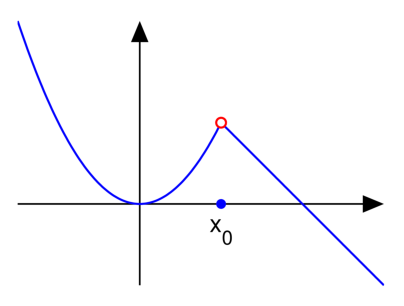
\includegraphics[scale=1.4]{figures/Discontinuity_removable}
        \caption{\centering Removable discontinuity}
    \label{fig:disc1}
\end{figure}



% Landscape page environment
\begin{landscape}

\subsection{Sub-figures, Sub-tables, and Landscape Pages}\label{subsec:landscape}
For the figures or tables that include sub-parts you can use \texttt{\textbackslash{begin\{subfigure\}}} within figure environment, as shown in this page to create and cite sub-figures, or similarly sub-tables. For instance, you can cite First sub-figure (see Figure~\ref{fig:suba}), and Second sub-figure (Figure~\ref{fig:subb}) or you can cite the whole figure as Figure~\ref{fig:subfigs}.

Notice that this is a landscape page and it has no page number. Sometimes when you have a large figure or a figure with multiple sub-figures that do not fit into the width of the page. In this case you may create a landscape page by using the \texttt{\textbackslash{begin\{landscape\}}} environment. Only write down the related content in this page and continue the rest of the thesis outside of the landscape page.

\begin{figure}
  \centering
  \begin{subfigure}[b]{0.4\textwidth}
    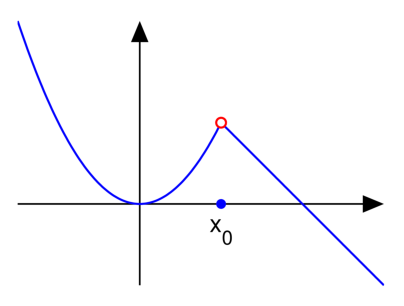
\includegraphics[width=\textwidth]{figures/Discontinuity_removable}
    \caption{First sub-figure}
    \label{fig:suba}
  \end{subfigure}
  \begin{subfigure}[b]{0.4\textwidth}
    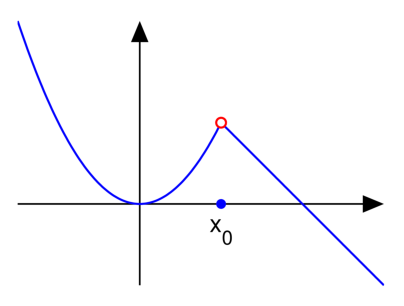
\includegraphics[width=\textwidth]{figures/Discontinuity_removable}
    \caption{Second sub-figure}
    \label{fig:subb}
  \end{subfigure}
  \begin{subfigure}[b]{0.4\textwidth}
    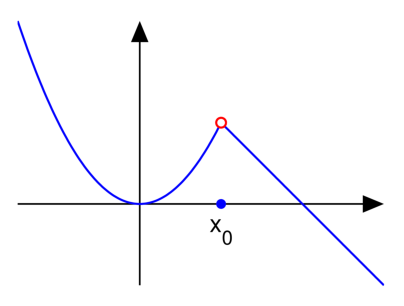
\includegraphics[width=\textwidth]{figures/Discontinuity_removable}
    \caption{Third sub-figure}
    \label{fig:subc}
  \end{subfigure}
  \vspace{6pt}
  \caption{Using sub-figures}
  \label{fig:subfigs}
\end{figure}

\end{landscape}

% ===== A3 Landscape page
%\KOMAoptions{paper=a3,BCOR=-14mm,DIV=12,paper=landscape,pagesize}
%\recalctypearea

%This is an A3 page.

%\begin{figure}[!ht]
%    \centering
%    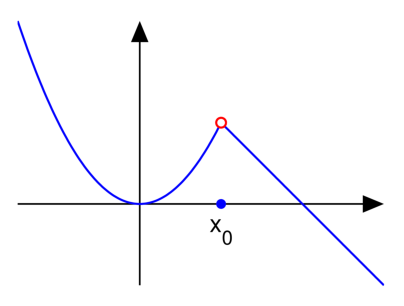
\includegraphics[scale=3]{figures/Discontinuity_removable}
%        \caption{\centering Removable discontinuity }
%    \label{fig:a3}
%\end{figure}

%\KOMAoptions{paper=a4,BCOR=15.7mm,paper=portrait,pagesize}
%\recalctypearea
% =====

\section{References}\label{sec:references}
For references you may use any standard style such as APA, IEEE, Chicago, etc. You have to be consistent with the citation and bibliography style throughout your entire thesis.

\section{Appendices (Optional)}\label{sec:appendices}
If available, you may use \texttt{appendix} or \texttt{appendices} environment. The former is used when you have only one appendix, and the former is used when you have multiple appendices which need to be separated as Appendix A, Appendix B, etc.

% --- Fork fix (see README "Fixes applied"): appendix tables/figures must not
% appear in the front-matter List of Tables / List of Figures. EMU_Thesis.tex
% sets \captionsetup[table]{list=no} and \captionsetup[figure]{list=no} right
% after \begin{appendices}, so nothing further is needed here -- just keep
% your appendix content inside that environment as normal.

\section{Index (Optional)}\label{sec:index}
Similar to appendices, if available, You may create index for your thesis by defining indices using \texttt{\textbackslash{index}\{\}} command in a proper place after the indexed word. For example if I use the command \texttt{\textbackslash{index}\{Index\}} exactly after the word index\index{Index}, it will appear in the INDEX section with its page number reference.

You can also create a nested index\index{Index!Nested Index} by prefixing the parent index word with ! mark to the child index. For example \texttt{\textbackslash{index}\{Index!Nested Index\}} will create a nested index.


%================== REFERENCES ==================
% You may either use thebibliography environment to manually
% add the references
%\begin{thebibliography}{2}
%\bibitem{igsr} "Writing Your Thesis, Defence and Graduation Procedures", \textit{Institute of Graduate Studies and Research - EMU}, 2020. [Online]. Available: %https://grad.emu.edu.tr/en/academic-issues/theses. [Accessed: 22- Jun- 2020].

%\bibitem{overleaf} "Overleaf, Online LaTeX Editor", \textit{Overleaf}, 2020. [Online]. Available: https://www.overleaf.com. [Accessed: 22- Jun- 2020].
%\end{thebibliography}

% or you may use a bibtex file with proper style
\bibliographystyle{IEEEtran}
\bibliography{references}

%================== APPENDIX / APPENDICES (if available) ==================
% Use 'appendix' or 'appendices' depending on your appendix contents
%\begin{appendix}
%    This is appendix with no specific sections.
%\end{appendix}

\begin{appendices}
% Fork fix: keep appendix tables/figures out of the front-matter lists.
\captionsetup[table]{list=no}
\captionsetup[figure]{list=no}

%    This is appendices with specific sections.

\appndxsec{Important Notes}{\label{app:importantnotes}}

You always need to use a blank line between paragraphs to indicate a new paragraph otherwise the compiler will merge the two paragraphs together as one. Refer to the \texttt{tex} file for demonstration.

Similarly, for equations you need to have a blank line before and after them, otherwise it will overlap with the previous paragraph.

The first paragraph of every chapter should be written under the chapter declaration without any extra line breaks; otherwise it will cause some spacing issues with the next section.

Contents below are for test only.

\begin{definition}[]
Let $U$ be the domain of discourse
\end{definition}

\begin{table}[htb] % [htb] to be after the paragraph
\caption{A table for the Appendix \ref{app:importantnotes} to test the appendix captions.}
\label{table:3}
\begin{tabular}{|c c c c|}
 \hline
 Col1 & Col2 & Col2 & Col3 \\ [0.5ex]
 \hline\hline
 1 & 6 & 87837 & 787 \\
 2 & 7 & 78 & 5415 \\
 3 & 545 & 778 & 7507 \\
 4 & 545 & 18744 & 7560 \\
 5 & 88 & 788 & 6344 \\ [1ex]
 \hline
\end{tabular}
\end{table}

\begin{equation}\label{eqa}
G_{\mu \nu }=8\pi GT_{\mu \nu }
\end{equation}

\appndxsec{Second Appendix with yet Another Really Long Title to Test Multi-line Titles}{\label{app:titlecheck}}

This appendix is solely for testing the table, figure, and equation numbering.

\begin{figure}[!b]
    \centering
    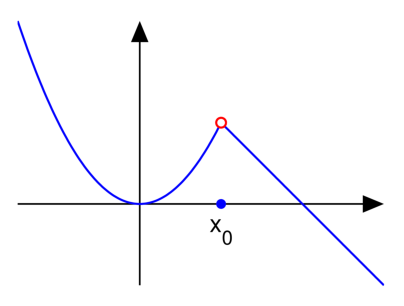
\includegraphics[scale=1.5]{figures/Discontinuity_removable}
        \caption{\centering Removable discontinuity, but it is scaled to 1.5 times the size of the original figure.}
    \label{fig:disc2}
\end{figure}

\begin{table}[b!] % [b!] to be at the bottom
\caption{Appendix \ref{app:titlecheck} table.}
\label{table:4}
\begin{tabular}{|c c c c|}
 \hline
 Col1 & Col2 & Col2 & Col3 \\ [0.5ex]
 \hline\hline
 1 & 6 & 87837 & 787 \\
 2 & 7 & 78 & 5415 \\
 3 & 545 & 778 & 7507 \\
 4 & 545 & 18744 & 7560 \\
 5 & 88 & 788 & 6344 \\ [1ex]
 \hline
\end{tabular}
\end{table}

\begin{equation}\label{eqb}
G_{\mu \nu }=8\pi GT_{\mu \nu }
\end{equation}

\begin{eqnarray}
  \sum \vert M^{\text{viol}}_g \vert ^2
   &=&  g^{2n-4}_S(Q^2)~N^{n-2} (N^2-1)
\nonumber
\\
   &&   \times \left( \sum_{i<j}\right) \sum_{\text{perm}}
            \frac{1}{S_{12}}  \frac{1}{S_{12}} \sum_\tau c^f_\tau
\,.
\label{eq:multilineeq2}
\end{eqnarray}

\begin{equation} \label{eu_eqn2}
e^{\pi i} + 1 = 0
\end{equation}

\begin{multline*}
p(x) = 3x^6 + 14x^5y + 590x^4y^2 + 19x^3y^3\\
- 12x^2y^4 - 12xy^5 + 2y^6 - a^3b^3
\end{multline*}

\begin{align*}
p(x) = 3x^6 + 14x^5y + 590x^4y^2 + 19x^3y^3\\
- 12x^2y^4 - 12xy^5 + 2y^6 - a^3b^3
\end{align*}

\begin{table}[htb]
\caption{Another appendix table.}
\label{table:5}
\begin{tabular}{|c c c c|}
 \hline
 Col1 & Col2 & Col2 & Col3 \\ [0.5ex]
 \hline\hline
 1 & 6 & 87837 & 787 \\
 2 & 7 & 78 & 5415 \\
 3 & 545 & 778 & 7507 \\
 4 & 545 & 18744 & 7560 \\
 5 & 88 & 788 & 6344 \\ [1ex]
 \hline
\end{tabular}
\end{table}

\end{appendices}

%================== INDEX (if available) ==================
\printindex

%############ End of Document (don't delete) ##############
\end{document}
"
% See README "Fixes applied" and EMU_Thesis.sty for the definitions.
% -----------------------------------------------------------------------

\begin{document}

% page numbering for the preliminary sections
\pagenumbering{roman}

% Justify text without hyphenation
% (You may disable this option but doing so may create problems in justifying paragraphs)
\tolerance=1
\emergencystretch=\maxdimen
\hyphenpenalty=10000
\hbadness=10000

%##################################################################
% Preliminary section
%##################################################################
%================== Title and Signature Pages =====================
\makethesistitle
\makeapprovalpage

%================== ABSTRACT ======================================
\begin{abstract}
Use this section to write down the abstract of your thesis. The length of the abstract must \textit{not} exceed 300 words. To keep the abstract short, avoid using too many introductory materials, and keep them for the introduction chapter.

At the end of the abstract, you need to provide 3 to 5 keywords related to the topic of your thesis. Keywords help others interested in your field to find your work more easily. The keywords need to be separated using a comma or a semicolon. Use the same separator for ÖZ as well.

% Every word of every keyword is capitalized automatically by \titlecap{}
% (format control checks for this). Just type the keywords in lowercase
% below and \titlecap{} takes care of the rest; it also correctly leaves
% acronyms/abbreviations you've already typed in caps (e.g. RAG) alone.
\noindent \textbf{Keywords}: \titlecap{keyword one, keyword two, ...}.
\end{abstract}

%================== ÖZ ============================================
\begin{ozet}
Tezinizin özetini yazmak için bu bölümü kullanın. Özetin uzunluğu 300 kelimeyi \textit{geçmemelidir}. Özeti kısa tutmak için çok fazla giriş materyali kullanmaktan kaçının ve bunları giriş bölümü için saklayın.

Özetin sonunda tezinizin konusu ile ilgili 3 - 5 anahtar kelime sağlamanız gerekmektedir. Anahtar kelimeler, alanınızla ilgilenen diğer kişilerin çalışmanızı daha kolay bulmasına yardımcı olur. Anahtar kelimelerin virgül veya noktalı virgül kullanılarak ayrılmalıdır. ABSTRACT için de aynı noktalama işaretini kullanınız. Her anahtar kelimenin ilk harfini büyük yazın (format kontrolü bunu denetler).

% \titlecap{} is NOT used here on purpose: it does not handle Turkish
% casing correctly (dotless "ı" is skipped entirely, and dotted "i" is
% wrongly capitalized to plain "I" instead of "İ", e.g. "iğne" wrongly
% becomes "Iğne" instead of "İğne"). Capitalize each Turkish keyword by
% hand and double-check dotted/dotless I's in the compiled PDF.
\noindent \textbf{Anahtar Kelimeler}: Anahtar Kelime Bir, Anahtar Kelime İki, ...
\end{ozet}

%================== DEDICATION (optional) =========================
\begin{notitlededication} %use {dedication} if you want the page title
\vspace{\fill}
\begin{center}
{\calligra... Dedicated to X} % you are not forced to use calligra font

The current page is using \texttt{notitlededication} for the Dedication page, this option will not print the title of this page. You may use the \texttt{dedication} if you want to include the title for this page. Also you may use any standard font face other than Times New Roman in this page.
\end{center}
\vspace{\fill}
\end{notitlededication}

%================== ACKNOWLEDGEMENTS (optional) ===================
\begin{acknowledgements}

In the acknowledgments section, you may express your gratitude towards others who helped you in completing your study and contributed to preparing your thesis.

Keep your acknowledgments section short and avoid going beyond one page.

\end{acknowledgements}

%================== PREFACE (optional) ============================
%\begin{preface}
% Preface is optional.
%\end{preface}

%================== TABLE OF CONTENTS =============================
\tableofcontents

%================== LIST OF TABLES (if available) =================
\listoftables

%================== LIST OF FIGURES (if available) ================
\listoffigures

%================== ABBREVIATIONS (if available) ==================
% For the list of symbols and abbreviations you have two options:
% 1. You can use nomencl package for the list of symbols and abbreviations. Follow the given example below:
% Note: use [aa] prefix before English symbols to force English letter symbols sorted at the beginning, and use [ab] prefix to sort Greek letter symbols afterward. For abbreviations you don't need to use any prefix.

%\nomenclature[aa]{$h$}{Planck constant}
%\nomenclature[aa]{$c$}{Speed of light in a vacuum inertial frame}
%\nomenclature[ab]{$\phi$}{Golden ratio}
%\nomenclature[ab]{$\mu$}{Micro sign}
%\nomenclature{sps}{Samples Per Second}
%\nomenclature{IMU}{Inertial Measurement Unit}
%\nomenclature{SoC}{System on Chip}
%\nomenclature{DMP}{Digital Motion Processor}
%\nomenclature{DSP}{Digital Signal Processor}
%\nomenclature{QFN}{Quad Flat No-leads}
%\nomenclature{LED}{Light-Emitting Diode}
%\nomenclature{GPIO}{General Purpose Input/Output}

%\printnomenclature


% 2. You can also use the below definitions for symbols and abbreviations instead of nomancl package (explained above). This way you can have separate list of symbols and list of abbreviations (optional).
% It is recommended to sort the list by an external software. The internal sorting function may not be accurate depending on the content.

% Create symbols
\DTLnewdb{symbols}
\addsymbol{$c$}{Speed of light in a vacuum inertial frame}
\addsymbol{$h$}{Planck constant}
\addsymbol[b]{$\mu$}{Micro sign}
\addsymbol[b]{$\phi$}{Golden ratio}

% Sort the list if needed
\DTLsort*{Acronym}{symbols}


% Create abbreviations
\DTLnewdb{abbreviation}
% Define the ABBREVIATIONS database as follows
\addabbreviation{sps}{ Samples Per Second}
\addabbreviation{IMU}{Inertial Measurement Unit}
\addabbreviation{SoC}{System on Chip}
\addabbreviation{DMP}{Digital Motion Processor}
\addabbreviation{DSP}{Digital Signal Processor}
\addabbreviation{QFN}{Quad Flat No-leads}
\addabbreviation{LED}{Light-Emitting Diode}
\addabbreviation{GPIO}{General Purpose Input/Output}

% Sort the list if needed
\DTLsort*{Acronym}{abbreviation}



% Use one of the page titles below depending on the content of your list:

\begin{symbolsandabbreviations}
  % Display the contents of the database
\end{symbolsandabbreviations}

%\begin{symbols}
  % Display the contents of the database
%\end{symbols}

%\begin{abbreviations}
  % Display the contents of the database
%\end{abbreviations}



%##################################################################
% End of the preliminary section
%##################################################################

% Begin the thesis body ==========================================
\clearpage
\pagenumbering{arabic} % page numbering for the thesis body

% Begin the FIRST CHAPTER =========================================
\chapter{INTRODUCTION}\label{ch:introduction}

\section{General Instructions}\label{sec:generalinstructions}
This \LaTeX~template is prepared and suggested  by the Institute of the Graduate Studies and Research (IGSR) for the graduating students who are willing to use \LaTeX~for their thesis report. The current version is a general template for engineering and mathematics programs. You may add other packages for any special input that is deemed necessary for your own thesis. However, the custom modifications need to be within the boundaries of the formatting guidelines\index{Guideline} provided by the IGSR. You may inquire your questions during format control sessions \cite{igsr}.

The current document is tested and works best with Overleaf\index{Overleaf} online \LaTeX~editor \cite{overleaf}. It has been tested on TeXstudio with Tex Live as well. One important note that you should be keeping in mind while working with this template is that, you always need to put an empty line break or \texttt{\textbackslash{par}} between your paragraphs or equations but not after the chapters or sections. Otherwise it may not work as intended and it would create some spacing issues.

\section{Chapters\index{Chapter} and Sections\index{Section}}\label{sec:chaptersnadsections}
Chapters and Section headings must be declared by \texttt{\textbackslash{chapter}}, \texttt{\textbackslash{section}}, \texttt{\textbackslash{subsection}}, and \texttt{\textbackslash{subsubsection}}. However, \texttt{\textbackslash{part}} and \texttt{\textbackslash{paragraph}} commands are not supported.

The title of the chapters should appear in $ALL~CAPITALS$, and the title of the sections can be either $Sentence~capital$ or $Initial~Capital$ but not both. All section titles must use justified alignment. Below is an example of \texttt{\textbackslash{subsection}}, and \texttt{\textbackslash{subsubsection}}:

\subsection{Subsection\index{Section!Subsection} Example with an Unusually Long Title That May Exceed a Single Line}\label{subsec:subsectionexample}
This is an example of how a subsection title should look like.

\subsubsection{Sub-subsection\index{Section!Sub-subsection} Example}\label{subsubsec:subsubsectionexample}
Here is an example of how a sub-subsection title should look like.

\section{Paragraphs}\label{sec:paragraphs}
Paragraphs can follow one of the following styles. Either indented at the first line with double spacing between every paragraph, or no indent but 24 pt space between every paragraph. The current template only supports the latter.

For paragraphs that end with `:', `;', or `,' the author must reduce the space between the current paragraph and the next paragraph to 0pt with double spacing. For this purpose you may use the \texttt{\textbackslash{noskip}} command at the end of your paragraph. Do not use the mentioned command if the paragraph is followed by an equation.

For example:\noskip
The space between the above line and this paragraph is reduced by \texttt{\textbackslash{noskip}} command because it is considered a continuation to the previous paragraph.

\subsection{Quotations\index{Quotation}}\label{subsec:quotations}

Quotation with more than 40 words or 3 lines need to be put in \texttt{quotation} environment with no paragraph spacing before the quotation. Below is an example of how a quotation should look like:

\noskip
\begin{quotation}
    Lorem ipsum, or lipsum as it is sometimes known, is dummy text used in laying out print, graphic or web designs. The passage is attributed to an unknown typesetter in the 15th century who is thought to have scrambled parts of Cicero's De Finibus Bonorum et Malorum for use in a type specimen book.
\end{quotation}

If there are several consequent quotations that are related together, you may use \texttt{\textbackslash{noskip}} between each of them.

\section{Equations}\label{sec:equations}

Equations can be generated using different environments. An empty line is always required before beginning your equation environment. Normally, the space between the equations and between the equation and its previous and next paragraphs is the same as the normal line skip. However, if necessary, the space after can be 24pt when the next paragraph is not related to the current equation. For this purpose, just place an empty line after the equation.

Some examples for equations are given below:

\begin{equation}\label{eq0}
G_{\mu \nu }=8\pi GT_{\mu \nu }
\end{equation}
where $G$ is the Newton constant, $G_{\mu \nu }$.

Equation Array:

\begin{eqnarray}
  \sum \vert M^{\text{viol}}_g \vert ^2
   &=&  g^{2n-4}_S(Q^2)~N^{n-2} (N^2-1)
\nonumber
\\
   &&   \times \left( \sum_{i<j}\right) \sum_{\text{perm}}
            \frac{1}{S_{12}}  \frac{1}{S_{12}} \sum_\tau c^f_\tau
\,.
\label{eq:multilineeq}
\end{eqnarray}
Use the following blocks to create your equations for the best results. If you encountered any issues, please report them to the format check office of the IGSR. Recommended equation formats are as follows: \noskip

Another simple Equation:

\begin{equation} \label{eu_eqn}
  e^{\pi i} + 1 = 0
\end{equation}
The beautiful equation \eqref{eu_eqn} is known as the Euler equation.

Long equations can be broken in several lines using the \texttt{split} environment from \textit{amsmath} package or using multi-line equation environment. For example, see the equation below.

\begin{equation}
p(x) = 3x^6 + 14x^5y + 590x^4y^2 + 19x^3y^3 - 12x^2y^4 - 12xy^5 + 2y^6 - a^3b^3 - 2a^2b^2 + 3x^3y^3
\end{equation}
Multi-line equation version:

\begin{multline}
p(x) = 3x^6 + 14x^5y + 590x^4y^2 + \\
  19x^3y^3 - 12x^2y^4 - 12xy^5 + \\
  2y^6 - a^3b^3 - 2a^2b^2 + 3x^3y^3
\end{multline}
Split equation version:

\begin{equation}
\begin{split}
p(x) = 3x^6 + 14x^5y + 590x^4y^2 + \\
19x^3y^3 - 12x^2y^4 - 12xy^5 + \\
2y^6 - a^3b^3 - 2a^2b^2 + 3x^3y^3
\end{split}
\end{equation}
Equation using align:

\begin{align*}
2x - 5y &=  8 \\
3x + 9y &=  -12
\end{align*}
Equation with nested aligned environment. This is for multi line equations with only one equation number using aligned nested in equation:

\begin{equation} \label{nested_eqn}
\begin{aligned}
x&=y           &  w &=z              &  a&=b+c\\
2x&=-y         &  3w&=\frac{1}{2}z   &  a&=b\\
-4 + 5x&=2+y   &  w+2&=-1+w          &  ab&=cb
\end{aligned}
\end{equation}
\filbreak %fillbreak is used when you want to keep the upcoming text together with the current text. For example here Grouping: with the next equation should be on the same page.
Grouping:

\begin{gather*}
2x - 5y =  8 \\
3x^2 + 9y =  3a + c
\end{gather*}

\section{Lists\index{List}}\label{sec:lists}
You can use the \texttt{\textbackslash{itemize}} environments for unordered lists\index{List!Unordered List} or \texttt{\textbackslash{enumerate}} command for ordered lists to generate lists.
% Use \noskip for paragraphs ending with ':', ';', and ','
% except when the next line is an equation
Unordered list\index{List!Unordered List} example:\noskip

\begin{itemize}
  \item One entry in the list,
  \item Another entry in the list.
\end{itemize}

Ordered\index{List!Ordered List} list example:\noskip

\begin{enumerate}
  \item The labels consists of sequential numbers.
  \item The numbers starts at 1 with every call to the enumerate environment.
\end{enumerate}

Ordered list\index{List!Ordered List} example with roman labels:\noskip
\begin{enumerate}[label=\roman*.]
  \item The labels consists of sequential numbers.
  \item The numbers starts at i with every call to the enumerate environment.
\end{enumerate}

Nested list\index{List!Nested List} example:\noskip

\begin{enumerate}
   \item The labels consists of sequential numbers.
   \begin{itemize}
     \item The individual entries are indicated with a black dot, a so-called bullet.
        \begin{equation} \label{eu_eqn_itemize}
          e^{\pi i} + 1 = 0
        \end{equation}
     \item The text in the entries may be of any length.
   \end{itemize}
   \item The numbers starts at 1 with every call to the enumerate environment.
\end{enumerate}

% Begin the SECOND CHAPTER =========================================
\chapter{PRELIMINARY SECTIONS, FIGURES, TABLES, AND REFERENCE MATERIALS}\label{ch:preliminary}
For the preliminary sections, please, refer to the comments written before every section environment in the \texttt{tex} file.\footnote{Comments start with a \% mark and usually have different color in the code editor.} For the list of symbols and abbreviations, the list has to be either sorted by the order of appearance or by alphabetic order. For the latter, symbols must be sorted first and then abbreviations, also, it should be sorted first by the order of English letters then Greek letters.

\section{Theorems, Definitions, Examples, etc.}\label{sec:theorems}
Currently, this template has support for remark\index{Remark}, definition\index{Definition}, preposition\index{Proposition}, conjecture\index{Conjecture}, theorem\index{Theorem}, lemma\index{Lemma}, and corollary\index{Corollary} sections. You may use the exact wording as mentioned for the environments. For instance, use \texttt{\textbackslash{begin\{definition\}[ ]}} for initiating a definition. Some examples are given below. \footnote{If you need a theorem style caption that is not listed here, you may create it yourself by following the appropriate style, or contact IGSR for help.}

\begin{remark}[Remark Name (optional)]
This is a Remark.
\end{remark}

\begin{definition}[Definition Name (optional)]
Let $U$ be the domain of discourse.
\end{definition}

\begin{eqnarray}
\label{fuzzy_set}
\tilde{A}=&\{(u,\mu_{\tilde{A}(u)})| u \in U\}
\nonumber
\\
&\mu_{\tilde{A}}:U \longrightarrow [0,1]
\,.
\end{eqnarray}

\begin{proposition}[Proposition Name (optional)]
This is a preposition.
\end{proposition}

\begin{conjecture}[Conjecture Name (optional)]
This is a Conjecture.
\end{conjecture}

\begin{example}[Example Name (optional)]
This is an example.
\end{example}

\begin{theorem}[Theorem Name (optional)]
This is a theorem.
\end{theorem}
\begin{proof}
Assume this is proof of the theorem.
\end{proof}


\begin{lemma}[Lemma Name (optional)]
This is a lemma.
\end{lemma}

\begin{corollary}[Corollary Name (optional)]
This is a corollary.
\end{corollary}

The numbering here is set to be based on the chapter\index{Chapter}. However, you ma change it to be based on the section as well.

\section{Tables and Figures}\label{sec:tablesandfigures}
Tables and figures are preferred to be on the top of the page unless it is necessary to be between certain paragraphs, or the bottom of the page. However, they should not appear stand alone in the middle of the page with no text, in this case it should be at the top of the page. It is a good practice to define multiple position choices and find the best option for your thesis. Figures have their caption under the figure, but table captions should be above the table.

% --- Fork fix (see README "Fixes applied"): table captions are left-aligned
% and figure captions are centered globally via \captionsetup in EMU_Thesis.tex,
% so \centering is no longer needed inside \caption{} for tables (and is
% redundant, though harmless, for figures). Caption text itself should be
% sentence case: only the first letter of the whole caption is capitalized;
% words that start a later sentence within the same caption stay lowercase
% unless they are proper nouns, abbreviations, or technical terms.
% Wide tables: give every column an explicit p{...} width. An unwrapped
% \texttt{l}/\texttt{c}/\texttt{r} column takes its natural (unwrapped) width from
% its widest cell, so one long entry can silently push the whole table past
% the right margin -- this is the single most common overflow bug students hit.
% Also format-control-checked: don't use manual \textbf{} for emphasis in
% running body text (paragraph prose, list-item leads such as "Term. Rest of
% the sentence...", or field labels in a structured listing). Use \emph{}
% instead, or leave it unstyled. \textbf{} is still fine where it isn't body
% text: table column headers, and labels inside a figure/diagram (e.g. a
% TikZ node). The bold "Keywords"/"Anahtar Kelimeler" line in the
% Abstract/ÖZ is a separate, standard front-matter convention, not body
% prose, and keeps its bold.

Table \ref{table:1} is defined to be immediately after its preceding paragraph, while, Table \ref{table:2} and Figure \ref{fig:disc1} are defined to be on top of the page.

\begin{table}
    \caption{First table to test placement.}
    \label{table:1}
    \begin{tabular}{|c c c c|}
     \hline
     Col1 & Col2 & Col2 & Col3 \\ [0.5ex]
     \hline\hline
     1 & 6 & 87837 & 787 \\
     2 & 7 & 78 & 5415 \\
     3 & 545 & 778 & 7507 \\
     4 & 545 & 18744 & 7560 \\
     5 & 88 & 788 & 6344 \\ [1ex]
     \hline
    \end{tabular}
\end{table}

\begin{table}[!htbp]
    \caption{Second table to test placement.}
    \label{table:2}
    \begin{tabular}{|c c c c|}
     \hline
     Col1 & Col2 & Col2 & Col3 \\ [0.5ex]
     \hline\hline
     1 & 6 & 87837 & 787 \\
     2 & 7 & 78 & 5415 \\
     3 & 545 & 778 & 7507 \\
     4 & 545 & 18744 & 7560 \\
     5 & 88 & 788 & 6344 \\ [1ex]
     \hline
    \end{tabular}
\end{table}

The Space between two tables, table and paragraph should be all 24pt. Meaning it should be the same as the space between two normal paragraphs.The best practice is to copy the codes that are currently used for figures and tables here to create your own content. It is recommended to have figures and tables either at the top or bottom of the page and not between paragraphs. However, if you have to do it please use [!htbp] tag.

\begin{figure}[!htbp]
    \centering
    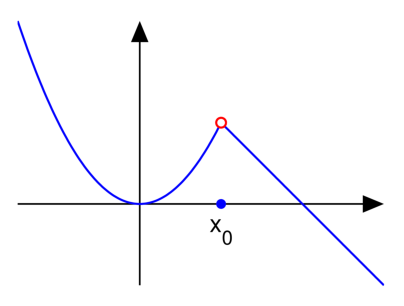
\includegraphics[scale=1.4]{figures/Discontinuity_removable}
        \caption{\centering Removable discontinuity}
    \label{fig:disc1}
\end{figure}



% Landscape page environment
\begin{landscape}

\subsection{Sub-figures, Sub-tables, and Landscape Pages}\label{subsec:landscape}
For the figures or tables that include sub-parts you can use \texttt{\textbackslash{begin\{subfigure\}}} within figure environment, as shown in this page to create and cite sub-figures, or similarly sub-tables. For instance, you can cite First sub-figure (see Figure~\ref{fig:suba}), and Second sub-figure (Figure~\ref{fig:subb}) or you can cite the whole figure as Figure~\ref{fig:subfigs}.

Notice that this is a landscape page and it has no page number. Sometimes when you have a large figure or a figure with multiple sub-figures that do not fit into the width of the page. In this case you may create a landscape page by using the \texttt{\textbackslash{begin\{landscape\}}} environment. Only write down the related content in this page and continue the rest of the thesis outside of the landscape page.

\begin{figure}
  \centering
  \begin{subfigure}[b]{0.4\textwidth}
    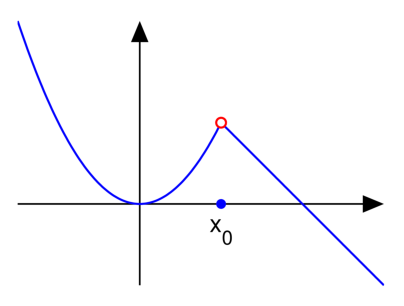
\includegraphics[width=\textwidth]{figures/Discontinuity_removable}
    \caption{First sub-figure}
    \label{fig:suba}
  \end{subfigure}
  \begin{subfigure}[b]{0.4\textwidth}
    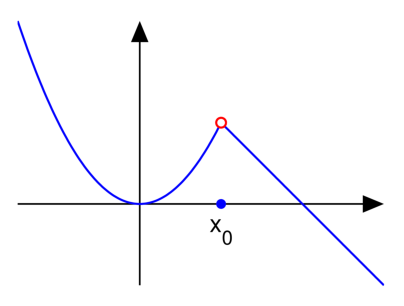
\includegraphics[width=\textwidth]{figures/Discontinuity_removable}
    \caption{Second sub-figure}
    \label{fig:subb}
  \end{subfigure}
  \begin{subfigure}[b]{0.4\textwidth}
    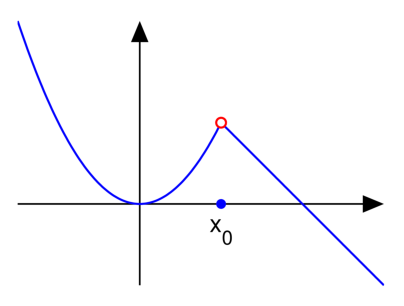
\includegraphics[width=\textwidth]{figures/Discontinuity_removable}
    \caption{Third sub-figure}
    \label{fig:subc}
  \end{subfigure}
  \vspace{6pt}
  \caption{Using sub-figures}
  \label{fig:subfigs}
\end{figure}

\end{landscape}

% ===== A3 Landscape page
%\KOMAoptions{paper=a3,BCOR=-14mm,DIV=12,paper=landscape,pagesize}
%\recalctypearea

%This is an A3 page.

%\begin{figure}[!ht]
%    \centering
%    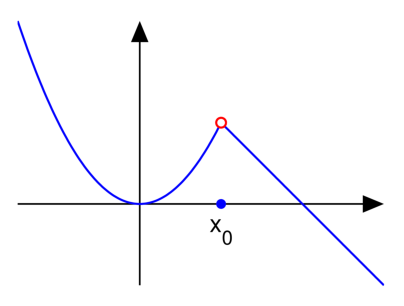
\includegraphics[scale=3]{figures/Discontinuity_removable}
%        \caption{\centering Removable discontinuity }
%    \label{fig:a3}
%\end{figure}

%\KOMAoptions{paper=a4,BCOR=15.7mm,paper=portrait,pagesize}
%\recalctypearea
% =====

\section{References}\label{sec:references}
For references you may use any standard style such as APA, IEEE, Chicago, etc. You have to be consistent with the citation and bibliography style throughout your entire thesis.

\section{Appendices (Optional)}\label{sec:appendices}
If available, you may use \texttt{appendix} or \texttt{appendices} environment. The former is used when you have only one appendix, and the former is used when you have multiple appendices which need to be separated as Appendix A, Appendix B, etc.

% --- Fork fix (see README "Fixes applied"): appendix tables/figures must not
% appear in the front-matter List of Tables / List of Figures. EMU_Thesis.tex
% sets \captionsetup[table]{list=no} and \captionsetup[figure]{list=no} right
% after \begin{appendices}, so nothing further is needed here -- just keep
% your appendix content inside that environment as normal.

\section{Index (Optional)}\label{sec:index}
Similar to appendices, if available, You may create index for your thesis by defining indices using \texttt{\textbackslash{index}\{\}} command in a proper place after the indexed word. For example if I use the command \texttt{\textbackslash{index}\{Index\}} exactly after the word index\index{Index}, it will appear in the INDEX section with its page number reference.

You can also create a nested index\index{Index!Nested Index} by prefixing the parent index word with ! mark to the child index. For example \texttt{\textbackslash{index}\{Index!Nested Index\}} will create a nested index.


%================== REFERENCES ==================
% You may either use thebibliography environment to manually
% add the references
%\begin{thebibliography}{2}
%\bibitem{igsr} "Writing Your Thesis, Defence and Graduation Procedures", \textit{Institute of Graduate Studies and Research - EMU}, 2020. [Online]. Available: %https://grad.emu.edu.tr/en/academic-issues/theses. [Accessed: 22- Jun- 2020].

%\bibitem{overleaf} "Overleaf, Online LaTeX Editor", \textit{Overleaf}, 2020. [Online]. Available: https://www.overleaf.com. [Accessed: 22- Jun- 2020].
%\end{thebibliography}

% or you may use a bibtex file with proper style
\bibliographystyle{IEEEtran}
\bibliography{references}

%================== APPENDIX / APPENDICES (if available) ==================
% Use 'appendix' or 'appendices' depending on your appendix contents
%\begin{appendix}
%    This is appendix with no specific sections.
%\end{appendix}

\begin{appendices}
% Fork fix: keep appendix tables/figures out of the front-matter lists.
\captionsetup[table]{list=no}
\captionsetup[figure]{list=no}

%    This is appendices with specific sections.

\appndxsec{Important Notes}{\label{app:importantnotes}}

You always need to use a blank line between paragraphs to indicate a new paragraph otherwise the compiler will merge the two paragraphs together as one. Refer to the \texttt{tex} file for demonstration.

Similarly, for equations you need to have a blank line before and after them, otherwise it will overlap with the previous paragraph.

The first paragraph of every chapter should be written under the chapter declaration without any extra line breaks; otherwise it will cause some spacing issues with the next section.

Contents below are for test only.

\begin{definition}[]
Let $U$ be the domain of discourse
\end{definition}

\begin{table}[htb] % [htb] to be after the paragraph
\caption{A table for the Appendix \ref{app:importantnotes} to test the appendix captions.}
\label{table:3}
\begin{tabular}{|c c c c|}
 \hline
 Col1 & Col2 & Col2 & Col3 \\ [0.5ex]
 \hline\hline
 1 & 6 & 87837 & 787 \\
 2 & 7 & 78 & 5415 \\
 3 & 545 & 778 & 7507 \\
 4 & 545 & 18744 & 7560 \\
 5 & 88 & 788 & 6344 \\ [1ex]
 \hline
\end{tabular}
\end{table}

\begin{equation}\label{eqa}
G_{\mu \nu }=8\pi GT_{\mu \nu }
\end{equation}

\appndxsec{Second Appendix with yet Another Really Long Title to Test Multi-line Titles}{\label{app:titlecheck}}

This appendix is solely for testing the table, figure, and equation numbering.

\begin{figure}[!b]
    \centering
    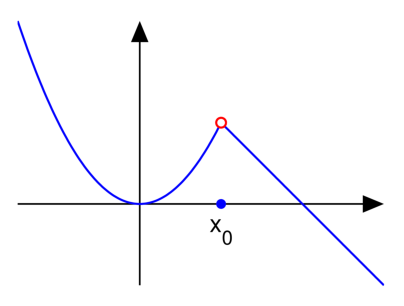
\includegraphics[scale=1.5]{figures/Discontinuity_removable}
        \caption{\centering Removable discontinuity, but it is scaled to 1.5 times the size of the original figure.}
    \label{fig:disc2}
\end{figure}

\begin{table}[b!] % [b!] to be at the bottom
\caption{Appendix \ref{app:titlecheck} table.}
\label{table:4}
\begin{tabular}{|c c c c|}
 \hline
 Col1 & Col2 & Col2 & Col3 \\ [0.5ex]
 \hline\hline
 1 & 6 & 87837 & 787 \\
 2 & 7 & 78 & 5415 \\
 3 & 545 & 778 & 7507 \\
 4 & 545 & 18744 & 7560 \\
 5 & 88 & 788 & 6344 \\ [1ex]
 \hline
\end{tabular}
\end{table}

\begin{equation}\label{eqb}
G_{\mu \nu }=8\pi GT_{\mu \nu }
\end{equation}

\begin{eqnarray}
  \sum \vert M^{\text{viol}}_g \vert ^2
   &=&  g^{2n-4}_S(Q^2)~N^{n-2} (N^2-1)
\nonumber
\\
   &&   \times \left( \sum_{i<j}\right) \sum_{\text{perm}}
            \frac{1}{S_{12}}  \frac{1}{S_{12}} \sum_\tau c^f_\tau
\,.
\label{eq:multilineeq2}
\end{eqnarray}

\begin{equation} \label{eu_eqn2}
e^{\pi i} + 1 = 0
\end{equation}

\begin{multline*}
p(x) = 3x^6 + 14x^5y + 590x^4y^2 + 19x^3y^3\\
- 12x^2y^4 - 12xy^5 + 2y^6 - a^3b^3
\end{multline*}

\begin{align*}
p(x) = 3x^6 + 14x^5y + 590x^4y^2 + 19x^3y^3\\
- 12x^2y^4 - 12xy^5 + 2y^6 - a^3b^3
\end{align*}

\begin{table}[htb]
\caption{Another appendix table.}
\label{table:5}
\begin{tabular}{|c c c c|}
 \hline
 Col1 & Col2 & Col2 & Col3 \\ [0.5ex]
 \hline\hline
 1 & 6 & 87837 & 787 \\
 2 & 7 & 78 & 5415 \\
 3 & 545 & 778 & 7507 \\
 4 & 545 & 18744 & 7560 \\
 5 & 88 & 788 & 6344 \\ [1ex]
 \hline
\end{tabular}
\end{table}

\end{appendices}

%================== INDEX (if available) ==================
\printindex

%############ End of Document (don't delete) ##############
\end{document}
"
% See README "Fixes applied" and EMU_Thesis.sty for the definitions.
% -----------------------------------------------------------------------

\begin{document}

% page numbering for the preliminary sections
\pagenumbering{roman}

% Justify text without hyphenation
% (You may disable this option but doing so may create problems in justifying paragraphs)
\tolerance=1
\emergencystretch=\maxdimen
\hyphenpenalty=10000
\hbadness=10000

%##################################################################
% Preliminary section
%##################################################################
%================== Title and Signature Pages =====================
\makethesistitle
\makeapprovalpage

%================== ABSTRACT ======================================
\begin{abstract}
Use this section to write down the abstract of your thesis. The length of the abstract must \textit{not} exceed 300 words. To keep the abstract short, avoid using too many introductory materials, and keep them for the introduction chapter.

At the end of the abstract, you need to provide 3 to 5 keywords related to the topic of your thesis. Keywords help others interested in your field to find your work more easily. The keywords need to be separated using a comma or a semicolon. Use the same separator for ÖZ as well.

% Every word of every keyword is capitalized automatically by \titlecap{}
% (format control checks for this). Just type the keywords in lowercase
% below and \titlecap{} takes care of the rest; it also correctly leaves
% acronyms/abbreviations you've already typed in caps (e.g. RAG) alone.
\noindent \textbf{Keywords}: \titlecap{keyword one, keyword two, ...}.
\end{abstract}

%================== ÖZ ============================================
\begin{ozet}
Tezinizin özetini yazmak için bu bölümü kullanın. Özetin uzunluğu 300 kelimeyi \textit{geçmemelidir}. Özeti kısa tutmak için çok fazla giriş materyali kullanmaktan kaçının ve bunları giriş bölümü için saklayın.

Özetin sonunda tezinizin konusu ile ilgili 3 - 5 anahtar kelime sağlamanız gerekmektedir. Anahtar kelimeler, alanınızla ilgilenen diğer kişilerin çalışmanızı daha kolay bulmasına yardımcı olur. Anahtar kelimelerin virgül veya noktalı virgül kullanılarak ayrılmalıdır. ABSTRACT için de aynı noktalama işaretini kullanınız. Her anahtar kelimenin ilk harfini büyük yazın (format kontrolü bunu denetler).

% \titlecap{} is NOT used here on purpose: it does not handle Turkish
% casing correctly (dotless "ı" is skipped entirely, and dotted "i" is
% wrongly capitalized to plain "I" instead of "İ", e.g. "iğne" wrongly
% becomes "Iğne" instead of "İğne"). Capitalize each Turkish keyword by
% hand and double-check dotted/dotless I's in the compiled PDF.
\noindent \textbf{Anahtar Kelimeler}: Anahtar Kelime Bir, Anahtar Kelime İki, ...
\end{ozet}

%================== DEDICATION (optional) =========================
\begin{notitlededication} %use {dedication} if you want the page title
\vspace{\fill}
\begin{center}
{\calligra... Dedicated to X} % you are not forced to use calligra font

The current page is using \texttt{notitlededication} for the Dedication page, this option will not print the title of this page. You may use the \texttt{dedication} if you want to include the title for this page. Also you may use any standard font face other than Times New Roman in this page.
\end{center}
\vspace{\fill}
\end{notitlededication}

%================== ACKNOWLEDGEMENTS (optional) ===================
\begin{acknowledgements}

In the acknowledgments section, you may express your gratitude towards others who helped you in completing your study and contributed to preparing your thesis.

Keep your acknowledgments section short and avoid going beyond one page.

\end{acknowledgements}

%================== PREFACE (optional) ============================
%\begin{preface}
% Preface is optional.
%\end{preface}

%================== TABLE OF CONTENTS =============================
\tableofcontents

%================== LIST OF TABLES (if available) =================
\listoftables

%================== LIST OF FIGURES (if available) ================
\listoffigures

%================== ABBREVIATIONS (if available) ==================
% For the list of symbols and abbreviations you have two options:
% 1. You can use nomencl package for the list of symbols and abbreviations. Follow the given example below:
% Note: use [aa] prefix before English symbols to force English letter symbols sorted at the beginning, and use [ab] prefix to sort Greek letter symbols afterward. For abbreviations you don't need to use any prefix.

%\nomenclature[aa]{$h$}{Planck constant}
%\nomenclature[aa]{$c$}{Speed of light in a vacuum inertial frame}
%\nomenclature[ab]{$\phi$}{Golden ratio}
%\nomenclature[ab]{$\mu$}{Micro sign}
%\nomenclature{sps}{Samples Per Second}
%\nomenclature{IMU}{Inertial Measurement Unit}
%\nomenclature{SoC}{System on Chip}
%\nomenclature{DMP}{Digital Motion Processor}
%\nomenclature{DSP}{Digital Signal Processor}
%\nomenclature{QFN}{Quad Flat No-leads}
%\nomenclature{LED}{Light-Emitting Diode}
%\nomenclature{GPIO}{General Purpose Input/Output}

%\printnomenclature


% 2. You can also use the below definitions for symbols and abbreviations instead of nomancl package (explained above). This way you can have separate list of symbols and list of abbreviations (optional).
% It is recommended to sort the list by an external software. The internal sorting function may not be accurate depending on the content.

% Create symbols
\DTLnewdb{symbols}
\addsymbol{$c$}{Speed of light in a vacuum inertial frame}
\addsymbol{$h$}{Planck constant}
\addsymbol[b]{$\mu$}{Micro sign}
\addsymbol[b]{$\phi$}{Golden ratio}

% Sort the list if needed
\DTLsort*{Acronym}{symbols}


% Create abbreviations
\DTLnewdb{abbreviation}
% Define the ABBREVIATIONS database as follows
\addabbreviation{sps}{ Samples Per Second}
\addabbreviation{IMU}{Inertial Measurement Unit}
\addabbreviation{SoC}{System on Chip}
\addabbreviation{DMP}{Digital Motion Processor}
\addabbreviation{DSP}{Digital Signal Processor}
\addabbreviation{QFN}{Quad Flat No-leads}
\addabbreviation{LED}{Light-Emitting Diode}
\addabbreviation{GPIO}{General Purpose Input/Output}

% Sort the list if needed
\DTLsort*{Acronym}{abbreviation}



% Use one of the page titles below depending on the content of your list:

\begin{symbolsandabbreviations}
  % Display the contents of the database
\end{symbolsandabbreviations}

%\begin{symbols}
  % Display the contents of the database
%\end{symbols}

%\begin{abbreviations}
  % Display the contents of the database
%\end{abbreviations}



%##################################################################
% End of the preliminary section
%##################################################################

% Begin the thesis body ==========================================
\clearpage
\pagenumbering{arabic} % page numbering for the thesis body

% Begin the FIRST CHAPTER =========================================
\chapter{INTRODUCTION}\label{ch:introduction}

\section{General Instructions}\label{sec:generalinstructions}
This \LaTeX~template is prepared and suggested  by the Institute of the Graduate Studies and Research (IGSR) for the graduating students who are willing to use \LaTeX~for their thesis report. The current version is a general template for engineering and mathematics programs. You may add other packages for any special input that is deemed necessary for your own thesis. However, the custom modifications need to be within the boundaries of the formatting guidelines\index{Guideline} provided by the IGSR. You may inquire your questions during format control sessions \cite{igsr}.

The current document is tested and works best with Overleaf\index{Overleaf} online \LaTeX~editor \cite{overleaf}. It has been tested on TeXstudio with Tex Live as well. One important note that you should be keeping in mind while working with this template is that, you always need to put an empty line break or \texttt{\textbackslash{par}} between your paragraphs or equations but not after the chapters or sections. Otherwise it may not work as intended and it would create some spacing issues.

\section{Chapters\index{Chapter} and Sections\index{Section}}\label{sec:chaptersnadsections}
Chapters and Section headings must be declared by \texttt{\textbackslash{chapter}}, \texttt{\textbackslash{section}}, \texttt{\textbackslash{subsection}}, and \texttt{\textbackslash{subsubsection}}. However, \texttt{\textbackslash{part}} and \texttt{\textbackslash{paragraph}} commands are not supported.

The title of the chapters should appear in $ALL~CAPITALS$, and the title of the sections can be either $Sentence~capital$ or $Initial~Capital$ but not both. All section titles must use justified alignment. Below is an example of \texttt{\textbackslash{subsection}}, and \texttt{\textbackslash{subsubsection}}:

\subsection{Subsection\index{Section!Subsection} Example with an Unusually Long Title That May Exceed a Single Line}\label{subsec:subsectionexample}
This is an example of how a subsection title should look like.

\subsubsection{Sub-subsection\index{Section!Sub-subsection} Example}\label{subsubsec:subsubsectionexample}
Here is an example of how a sub-subsection title should look like.

\section{Paragraphs}\label{sec:paragraphs}
Paragraphs can follow one of the following styles. Either indented at the first line with double spacing between every paragraph, or no indent but 24 pt space between every paragraph. The current template only supports the latter.

For paragraphs that end with `:', `;', or `,' the author must reduce the space between the current paragraph and the next paragraph to 0pt with double spacing. For this purpose you may use the \texttt{\textbackslash{noskip}} command at the end of your paragraph. Do not use the mentioned command if the paragraph is followed by an equation.

For example:\noskip
The space between the above line and this paragraph is reduced by \texttt{\textbackslash{noskip}} command because it is considered a continuation to the previous paragraph.

\subsection{Quotations\index{Quotation}}\label{subsec:quotations}

Quotation with more than 40 words or 3 lines need to be put in \texttt{quotation} environment with no paragraph spacing before the quotation. Below is an example of how a quotation should look like:

\noskip
\begin{quotation}
    Lorem ipsum, or lipsum as it is sometimes known, is dummy text used in laying out print, graphic or web designs. The passage is attributed to an unknown typesetter in the 15th century who is thought to have scrambled parts of Cicero's De Finibus Bonorum et Malorum for use in a type specimen book.
\end{quotation}

If there are several consequent quotations that are related together, you may use \texttt{\textbackslash{noskip}} between each of them.

\section{Equations}\label{sec:equations}

Equations can be generated using different environments. An empty line is always required before beginning your equation environment. Normally, the space between the equations and between the equation and its previous and next paragraphs is the same as the normal line skip. However, if necessary, the space after can be 24pt when the next paragraph is not related to the current equation. For this purpose, just place an empty line after the equation.

Some examples for equations are given below:

\begin{equation}\label{eq0}
G_{\mu \nu }=8\pi GT_{\mu \nu }
\end{equation}
where $G$ is the Newton constant, $G_{\mu \nu }$.

Equation Array:

\begin{eqnarray}
  \sum \vert M^{\text{viol}}_g \vert ^2
   &=&  g^{2n-4}_S(Q^2)~N^{n-2} (N^2-1)
\nonumber
\\
   &&   \times \left( \sum_{i<j}\right) \sum_{\text{perm}}
            \frac{1}{S_{12}}  \frac{1}{S_{12}} \sum_\tau c^f_\tau
\,.
\label{eq:multilineeq}
\end{eqnarray}
Use the following blocks to create your equations for the best results. If you encountered any issues, please report them to the format check office of the IGSR. Recommended equation formats are as follows: \noskip

Another simple Equation:

\begin{equation} \label{eu_eqn}
  e^{\pi i} + 1 = 0
\end{equation}
The beautiful equation \eqref{eu_eqn} is known as the Euler equation.

Long equations can be broken in several lines using the \texttt{split} environment from \textit{amsmath} package or using multi-line equation environment. For example, see the equation below.

\begin{equation}
p(x) = 3x^6 + 14x^5y + 590x^4y^2 + 19x^3y^3 - 12x^2y^4 - 12xy^5 + 2y^6 - a^3b^3 - 2a^2b^2 + 3x^3y^3
\end{equation}
Multi-line equation version:

\begin{multline}
p(x) = 3x^6 + 14x^5y + 590x^4y^2 + \\
  19x^3y^3 - 12x^2y^4 - 12xy^5 + \\
  2y^6 - a^3b^3 - 2a^2b^2 + 3x^3y^3
\end{multline}
Split equation version:

\begin{equation}
\begin{split}
p(x) = 3x^6 + 14x^5y + 590x^4y^2 + \\
19x^3y^3 - 12x^2y^4 - 12xy^5 + \\
2y^6 - a^3b^3 - 2a^2b^2 + 3x^3y^3
\end{split}
\end{equation}
Equation using align:

\begin{align*}
2x - 5y &=  8 \\
3x + 9y &=  -12
\end{align*}
Equation with nested aligned environment. This is for multi line equations with only one equation number using aligned nested in equation:

\begin{equation} \label{nested_eqn}
\begin{aligned}
x&=y           &  w &=z              &  a&=b+c\\
2x&=-y         &  3w&=\frac{1}{2}z   &  a&=b\\
-4 + 5x&=2+y   &  w+2&=-1+w          &  ab&=cb
\end{aligned}
\end{equation}
\filbreak %fillbreak is used when you want to keep the upcoming text together with the current text. For example here Grouping: with the next equation should be on the same page.
Grouping:

\begin{gather*}
2x - 5y =  8 \\
3x^2 + 9y =  3a + c
\end{gather*}

\section{Lists\index{List}}\label{sec:lists}
You can use the \texttt{\textbackslash{itemize}} environments for unordered lists\index{List!Unordered List} or \texttt{\textbackslash{enumerate}} command for ordered lists to generate lists.
% Use \noskip for paragraphs ending with ':', ';', and ','
% except when the next line is an equation
Unordered list\index{List!Unordered List} example:\noskip

\begin{itemize}
  \item One entry in the list,
  \item Another entry in the list.
\end{itemize}

Ordered\index{List!Ordered List} list example:\noskip

\begin{enumerate}
  \item The labels consists of sequential numbers.
  \item The numbers starts at 1 with every call to the enumerate environment.
\end{enumerate}

Ordered list\index{List!Ordered List} example with roman labels:\noskip
\begin{enumerate}[label=\roman*.]
  \item The labels consists of sequential numbers.
  \item The numbers starts at i with every call to the enumerate environment.
\end{enumerate}

Nested list\index{List!Nested List} example:\noskip

\begin{enumerate}
   \item The labels consists of sequential numbers.
   \begin{itemize}
     \item The individual entries are indicated with a black dot, a so-called bullet.
        \begin{equation} \label{eu_eqn_itemize}
          e^{\pi i} + 1 = 0
        \end{equation}
     \item The text in the entries may be of any length.
   \end{itemize}
   \item The numbers starts at 1 with every call to the enumerate environment.
\end{enumerate}

% Begin the SECOND CHAPTER =========================================
\chapter{PRELIMINARY SECTIONS, FIGURES, TABLES, AND REFERENCE MATERIALS}\label{ch:preliminary}
For the preliminary sections, please, refer to the comments written before every section environment in the \texttt{tex} file.\footnote{Comments start with a \% mark and usually have different color in the code editor.} For the list of symbols and abbreviations, the list has to be either sorted by the order of appearance or by alphabetic order. For the latter, symbols must be sorted first and then abbreviations, also, it should be sorted first by the order of English letters then Greek letters.

\section{Theorems, Definitions, Examples, etc.}\label{sec:theorems}
Currently, this template has support for remark\index{Remark}, definition\index{Definition}, preposition\index{Proposition}, conjecture\index{Conjecture}, theorem\index{Theorem}, lemma\index{Lemma}, and corollary\index{Corollary} sections. You may use the exact wording as mentioned for the environments. For instance, use \texttt{\textbackslash{begin\{definition\}[ ]}} for initiating a definition. Some examples are given below. \footnote{If you need a theorem style caption that is not listed here, you may create it yourself by following the appropriate style, or contact IGSR for help.}

\begin{remark}[Remark Name (optional)]
This is a Remark.
\end{remark}

\begin{definition}[Definition Name (optional)]
Let $U$ be the domain of discourse.
\end{definition}

\begin{eqnarray}
\label{fuzzy_set}
\tilde{A}=&\{(u,\mu_{\tilde{A}(u)})| u \in U\}
\nonumber
\\
&\mu_{\tilde{A}}:U \longrightarrow [0,1]
\,.
\end{eqnarray}

\begin{proposition}[Proposition Name (optional)]
This is a preposition.
\end{proposition}

\begin{conjecture}[Conjecture Name (optional)]
This is a Conjecture.
\end{conjecture}

\begin{example}[Example Name (optional)]
This is an example.
\end{example}

\begin{theorem}[Theorem Name (optional)]
This is a theorem.
\end{theorem}
\begin{proof}
Assume this is proof of the theorem.
\end{proof}


\begin{lemma}[Lemma Name (optional)]
This is a lemma.
\end{lemma}

\begin{corollary}[Corollary Name (optional)]
This is a corollary.
\end{corollary}

The numbering here is set to be based on the chapter\index{Chapter}. However, you ma change it to be based on the section as well.

\section{Tables and Figures}\label{sec:tablesandfigures}
Tables and figures are preferred to be on the top of the page unless it is necessary to be between certain paragraphs, or the bottom of the page. However, they should not appear stand alone in the middle of the page with no text, in this case it should be at the top of the page. It is a good practice to define multiple position choices and find the best option for your thesis. Figures have their caption under the figure, but table captions should be above the table.

% --- Fork fix (see README "Fixes applied"): table captions are left-aligned
% and figure captions are centered globally via \captionsetup in EMU_Thesis.tex,
% so \centering is no longer needed inside \caption{} for tables (and is
% redundant, though harmless, for figures). Caption text itself should be
% sentence case: only the first letter of the whole caption is capitalized;
% words that start a later sentence within the same caption stay lowercase
% unless they are proper nouns, abbreviations, or technical terms.
% Wide tables: give every column an explicit p{...} width. An unwrapped
% \texttt{l}/\texttt{c}/\texttt{r} column takes its natural (unwrapped) width from
% its widest cell, so one long entry can silently push the whole table past
% the right margin -- this is the single most common overflow bug students hit.
% Also format-control-checked: don't use manual \textbf{} for emphasis in
% running body text (paragraph prose, list-item leads such as "Term. Rest of
% the sentence...", or field labels in a structured listing). Use \emph{}
% instead, or leave it unstyled. \textbf{} is still fine where it isn't body
% text: table column headers, and labels inside a figure/diagram (e.g. a
% TikZ node). The bold "Keywords"/"Anahtar Kelimeler" line in the
% Abstract/ÖZ is a separate, standard front-matter convention, not body
% prose, and keeps its bold.

Table \ref{table:1} is defined to be immediately after its preceding paragraph, while, Table \ref{table:2} and Figure \ref{fig:disc1} are defined to be on top of the page.

\begin{table}
    \caption{First table to test placement.}
    \label{table:1}
    \begin{tabular}{|c c c c|}
     \hline
     Col1 & Col2 & Col2 & Col3 \\ [0.5ex]
     \hline\hline
     1 & 6 & 87837 & 787 \\
     2 & 7 & 78 & 5415 \\
     3 & 545 & 778 & 7507 \\
     4 & 545 & 18744 & 7560 \\
     5 & 88 & 788 & 6344 \\ [1ex]
     \hline
    \end{tabular}
\end{table}

\begin{table}[!htbp]
    \caption{Second table to test placement.}
    \label{table:2}
    \begin{tabular}{|c c c c|}
     \hline
     Col1 & Col2 & Col2 & Col3 \\ [0.5ex]
     \hline\hline
     1 & 6 & 87837 & 787 \\
     2 & 7 & 78 & 5415 \\
     3 & 545 & 778 & 7507 \\
     4 & 545 & 18744 & 7560 \\
     5 & 88 & 788 & 6344 \\ [1ex]
     \hline
    \end{tabular}
\end{table}

The Space between two tables, table and paragraph should be all 24pt. Meaning it should be the same as the space between two normal paragraphs.The best practice is to copy the codes that are currently used for figures and tables here to create your own content. It is recommended to have figures and tables either at the top or bottom of the page and not between paragraphs. However, if you have to do it please use [!htbp] tag.

\begin{figure}[!htbp]
    \centering
    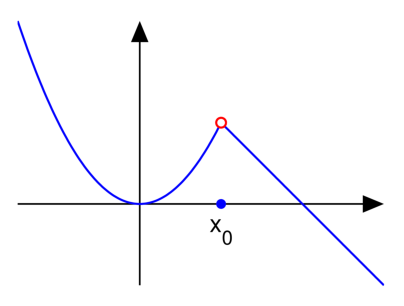
\includegraphics[scale=1.4]{figures/Discontinuity_removable}
        \caption{\centering Removable discontinuity}
    \label{fig:disc1}
\end{figure}



% Landscape page environment
\begin{landscape}

\subsection{Sub-figures, Sub-tables, and Landscape Pages}\label{subsec:landscape}
For the figures or tables that include sub-parts you can use \texttt{\textbackslash{begin\{subfigure\}}} within figure environment, as shown in this page to create and cite sub-figures, or similarly sub-tables. For instance, you can cite First sub-figure (see Figure~\ref{fig:suba}), and Second sub-figure (Figure~\ref{fig:subb}) or you can cite the whole figure as Figure~\ref{fig:subfigs}.

Notice that this is a landscape page and it has no page number. Sometimes when you have a large figure or a figure with multiple sub-figures that do not fit into the width of the page. In this case you may create a landscape page by using the \texttt{\textbackslash{begin\{landscape\}}} environment. Only write down the related content in this page and continue the rest of the thesis outside of the landscape page.

\begin{figure}
  \centering
  \begin{subfigure}[b]{0.4\textwidth}
    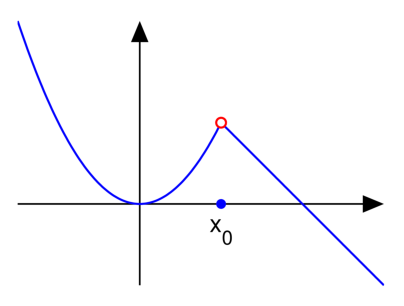
\includegraphics[width=\textwidth]{figures/Discontinuity_removable}
    \caption{First sub-figure}
    \label{fig:suba}
  \end{subfigure}
  \begin{subfigure}[b]{0.4\textwidth}
    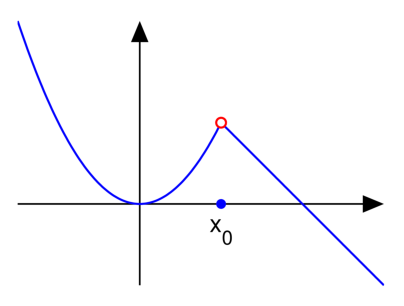
\includegraphics[width=\textwidth]{figures/Discontinuity_removable}
    \caption{Second sub-figure}
    \label{fig:subb}
  \end{subfigure}
  \begin{subfigure}[b]{0.4\textwidth}
    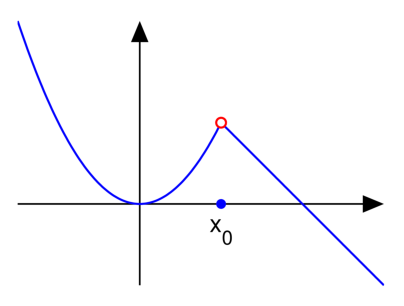
\includegraphics[width=\textwidth]{figures/Discontinuity_removable}
    \caption{Third sub-figure}
    \label{fig:subc}
  \end{subfigure}
  \vspace{6pt}
  \caption{Using sub-figures}
  \label{fig:subfigs}
\end{figure}

\end{landscape}

% ===== A3 Landscape page
%\KOMAoptions{paper=a3,BCOR=-14mm,DIV=12,paper=landscape,pagesize}
%\recalctypearea

%This is an A3 page.

%\begin{figure}[!ht]
%    \centering
%    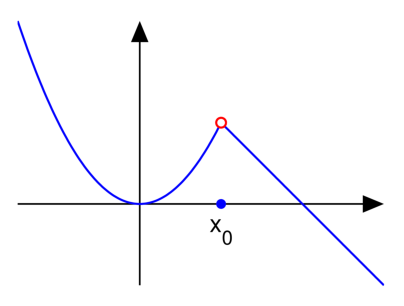
\includegraphics[scale=3]{figures/Discontinuity_removable}
%        \caption{\centering Removable discontinuity }
%    \label{fig:a3}
%\end{figure}

%\KOMAoptions{paper=a4,BCOR=15.7mm,paper=portrait,pagesize}
%\recalctypearea
% =====

\section{References}\label{sec:references}
For references you may use any standard style such as APA, IEEE, Chicago, etc. You have to be consistent with the citation and bibliography style throughout your entire thesis.

\section{Appendices (Optional)}\label{sec:appendices}
If available, you may use \texttt{appendix} or \texttt{appendices} environment. The former is used when you have only one appendix, and the former is used when you have multiple appendices which need to be separated as Appendix A, Appendix B, etc.

% --- Fork fix (see README "Fixes applied"): appendix tables/figures must not
% appear in the front-matter List of Tables / List of Figures. EMU_Thesis.tex
% sets \captionsetup[table]{list=no} and \captionsetup[figure]{list=no} right
% after \begin{appendices}, so nothing further is needed here -- just keep
% your appendix content inside that environment as normal.

\section{Index (Optional)}\label{sec:index}
Similar to appendices, if available, You may create index for your thesis by defining indices using \texttt{\textbackslash{index}\{\}} command in a proper place after the indexed word. For example if I use the command \texttt{\textbackslash{index}\{Index\}} exactly after the word index\index{Index}, it will appear in the INDEX section with its page number reference.

You can also create a nested index\index{Index!Nested Index} by prefixing the parent index word with ! mark to the child index. For example \texttt{\textbackslash{index}\{Index!Nested Index\}} will create a nested index.


%================== REFERENCES ==================
% You may either use thebibliography environment to manually
% add the references
%\begin{thebibliography}{2}
%\bibitem{igsr} "Writing Your Thesis, Defence and Graduation Procedures", \textit{Institute of Graduate Studies and Research - EMU}, 2020. [Online]. Available: %https://grad.emu.edu.tr/en/academic-issues/theses. [Accessed: 22- Jun- 2020].

%\bibitem{overleaf} "Overleaf, Online LaTeX Editor", \textit{Overleaf}, 2020. [Online]. Available: https://www.overleaf.com. [Accessed: 22- Jun- 2020].
%\end{thebibliography}

% or you may use a bibtex file with proper style
\bibliographystyle{IEEEtran}
\bibliography{references}

%================== APPENDIX / APPENDICES (if available) ==================
% Use 'appendix' or 'appendices' depending on your appendix contents
%\begin{appendix}
%    This is appendix with no specific sections.
%\end{appendix}

\begin{appendices}
% Fork fix: keep appendix tables/figures out of the front-matter lists.
\captionsetup[table]{list=no}
\captionsetup[figure]{list=no}

%    This is appendices with specific sections.

\appndxsec{Important Notes}{\label{app:importantnotes}}

You always need to use a blank line between paragraphs to indicate a new paragraph otherwise the compiler will merge the two paragraphs together as one. Refer to the \texttt{tex} file for demonstration.

Similarly, for equations you need to have a blank line before and after them, otherwise it will overlap with the previous paragraph.

The first paragraph of every chapter should be written under the chapter declaration without any extra line breaks; otherwise it will cause some spacing issues with the next section.

Contents below are for test only.

\begin{definition}[]
Let $U$ be the domain of discourse
\end{definition}

\begin{table}[htb] % [htb] to be after the paragraph
\caption{A table for the Appendix \ref{app:importantnotes} to test the appendix captions.}
\label{table:3}
\begin{tabular}{|c c c c|}
 \hline
 Col1 & Col2 & Col2 & Col3 \\ [0.5ex]
 \hline\hline
 1 & 6 & 87837 & 787 \\
 2 & 7 & 78 & 5415 \\
 3 & 545 & 778 & 7507 \\
 4 & 545 & 18744 & 7560 \\
 5 & 88 & 788 & 6344 \\ [1ex]
 \hline
\end{tabular}
\end{table}

\begin{equation}\label{eqa}
G_{\mu \nu }=8\pi GT_{\mu \nu }
\end{equation}

\appndxsec{Second Appendix with yet Another Really Long Title to Test Multi-line Titles}{\label{app:titlecheck}}

This appendix is solely for testing the table, figure, and equation numbering.

\begin{figure}[!b]
    \centering
    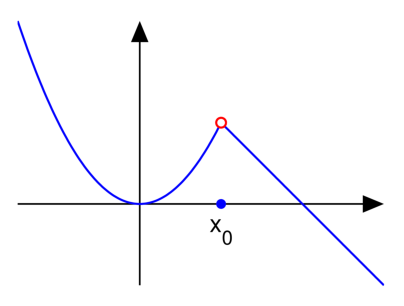
\includegraphics[scale=1.5]{figures/Discontinuity_removable}
        \caption{\centering Removable discontinuity, but it is scaled to 1.5 times the size of the original figure.}
    \label{fig:disc2}
\end{figure}

\begin{table}[b!] % [b!] to be at the bottom
\caption{Appendix \ref{app:titlecheck} table.}
\label{table:4}
\begin{tabular}{|c c c c|}
 \hline
 Col1 & Col2 & Col2 & Col3 \\ [0.5ex]
 \hline\hline
 1 & 6 & 87837 & 787 \\
 2 & 7 & 78 & 5415 \\
 3 & 545 & 778 & 7507 \\
 4 & 545 & 18744 & 7560 \\
 5 & 88 & 788 & 6344 \\ [1ex]
 \hline
\end{tabular}
\end{table}

\begin{equation}\label{eqb}
G_{\mu \nu }=8\pi GT_{\mu \nu }
\end{equation}

\begin{eqnarray}
  \sum \vert M^{\text{viol}}_g \vert ^2
   &=&  g^{2n-4}_S(Q^2)~N^{n-2} (N^2-1)
\nonumber
\\
   &&   \times \left( \sum_{i<j}\right) \sum_{\text{perm}}
            \frac{1}{S_{12}}  \frac{1}{S_{12}} \sum_\tau c^f_\tau
\,.
\label{eq:multilineeq2}
\end{eqnarray}

\begin{equation} \label{eu_eqn2}
e^{\pi i} + 1 = 0
\end{equation}

\begin{multline*}
p(x) = 3x^6 + 14x^5y + 590x^4y^2 + 19x^3y^3\\
- 12x^2y^4 - 12xy^5 + 2y^6 - a^3b^3
\end{multline*}

\begin{align*}
p(x) = 3x^6 + 14x^5y + 590x^4y^2 + 19x^3y^3\\
- 12x^2y^4 - 12xy^5 + 2y^6 - a^3b^3
\end{align*}

\begin{table}[htb]
\caption{Another appendix table.}
\label{table:5}
\begin{tabular}{|c c c c|}
 \hline
 Col1 & Col2 & Col2 & Col3 \\ [0.5ex]
 \hline\hline
 1 & 6 & 87837 & 787 \\
 2 & 7 & 78 & 5415 \\
 3 & 545 & 778 & 7507 \\
 4 & 545 & 18744 & 7560 \\
 5 & 88 & 788 & 6344 \\ [1ex]
 \hline
\end{tabular}
\end{table}

\end{appendices}

%================== INDEX (if available) ==================
\printindex

%############ End of Document (don't delete) ##############
\end{document}
